% ---------------------------------------------------------
% Vorlage abschlussarbeit.tex
%
% Erstellen: pdflatex, biber, pdflatex, pdflatex
%
% Formatierung für doppelseitigen Druck (dringend empfohlen)
%
% Nutzungshinweis zum Hochschullogo:
%
% Das Logo kann, muss aber nicht auf der Titelseite der Abschlussarbeit
% stehen. Größe und Position des Logos sollen nicht verändert werden; die
% Überlappung mit dem Text ist beabsichtigt. Die Erlaubnis zur Nutzung des
% Logos erstreckt sich nur auf die Abschlussarbeit.
%
% Volker Ahlers, Hochschule Hannover, 2013-2020
% ---------------------------------------------------------

\documentclass[11pt,DIV=12,BCOR=0mm,twoside,openright,headings=normal,%
  numbers=noenddot,headsepline,headinclude]{scrreprt}
\usepackage[automark,headsepline]{scrlayer-scrpage}
\usepackage[utf8]{inputenc}         % UTF8 encoding
\usepackage[T1]{fontenc}
\usepackage{newtxtext,newtxmath}
\usepackage[english]{babel}
\usepackage[fixlanguage]{babelbib}
\usepackage{graphicx}
\usepackage[usenames]{xcolor}
\usepackage{listings}
\usepackage[pdftex]{hyperref}
\usepackage{wallpaper}
\usepackage{physics}
\usepackage{amsmath}
%\usepackage{amssymb}
\usepackage{tikz}
\usepackage{wrapfig}
\usepackage[list=true]{subcaption}
\usepackage[cache=false]{minted}
\usepackage{scrhack}
\usepackage{hhline}
\usepackage{varwidth}
\usepackage{booktabs}
\usepackage{caption}
\usepackage{siunitx}
\usepackage{cases}
\usepackage{needspace}

% You can change the style for code blocks here. See: https://www.overleaf.com/learn/latex/Code_Highlighting_with_minted
\usemintedstyle{rainbow_dash}
\setminted{
linenos,
autogobble,
fontsize=\footnotesize,
breaklines
}

\setcapindent{15pt}

% You can declare your own units here.
\DeclareSIUnit\px{px}
\DeclareSIUnit\atm{atm}
\DeclareSIUnit\AU{AU}

\KOMAoptions{headinclude}
\hypersetup{linkcolor=black,pdfborder=0 0 0}

\tolerance=2000
\emergencystretch 20pt
\frenchspacing

\begin{document}

    \selectlanguage{english}
    \selectbiblanguage{english}

    \thispagestyle{empty}
    \pagenumbering{roman}

    \newlength{\DLROffset}
    \setlength{\DLROffset}{0.05\paperheight}
    \AddToShipoutPicture*{
        \AtPageUpperLeft{
            \raisebox{-\height - \DLROffset}{
                \hspace{\DLROffset}
                
\includegraphics[height=0.13\paperheight]{DLR_Logo.png}
            }
        }
    }

    \newlength{\HsHOffset}
    \setlength{\HsHOffset}{0.05\paperheight}
    \AddToShipoutPicture*{
        \AtPageLowerLeft{
            \parbox[b]{\paperwidth - \HsHOffset}{
                \hfill
                
\includegraphics[height=0.33\paperheight]{hsh-logo}
                \vspace*{\HsHOffset}
            }
        }
    }

    \begin{center}
        \vspace*{4\baselineskip}
        {\sffamily\bfseries\LARGE
        Motion Sickness Reduction for 6-DoF-Navigation in a Virtual Solar System\par}

        \vspace*{4\baselineskip}
        {\Large Moritz Zeumer}

        \vfill
        {\Large Master Thesis}

        \vspace*{4\baselineskip}
        {\Large Hochschule Hannover\\
        Faculty IV -- Business and Computer Science\\
        Course of Studies M.\,Sc.\ Applied Computer Sciences\par}

        \vspace*{4\baselineskip}
        {\Large \today}

        \vspace*{4\baselineskip}
    \end{center}

    \cleardoublepage

    \noindent
    {\sffamily\bfseries Author}

    \vspace*{.5\baselineskip}
    \noindent
    Moritz Zeumer\\
    Matrikelnummer: 1498947\\
    E-Mail: M\_Zeumer@gmx.de

    \vspace*{1\baselineskip}
    \noindent
    {\sffamily\bfseries Examiner}

    \vspace*{.5\baselineskip}
    \noindent
    Prof. Dr. Volker Ahlers\\
    Hochschule Hannover\\
    Faculty IV, Computer Science\\
    Ricklinger Stadtweg 120\\
    30459 Hannover

    \vspace*{1\baselineskip}
    \noindent
    {\sffamily\bfseries Second Examiner}

    \vspace*{.5\baselineskip}
    \noindent
    M. Sc. Simon Schneegans\\
    German Aerospace Center (DLR)\\
    Institute for Software Technology\\
    Software for Space Systems and Interactive Visualization\\
    Lilienthalplatz 7\\
    38108 Braunschweig

    \vfill
    \noindent
    {\sffamily\bfseries Declaration of Authorship}

    \vspace*{.5\baselineskip}
    \noindent
    I hereby declare that this thesis, and the work presented in it are my own and has been generated by me as the result of my own original research.
    I confirm that:

    \begin{enumerate}
        \item Where I have consulted the published work of others, this is always clearly attributed.

        \item Where I have quoted from the work of others, the source is always given.
        Except for such quotations, this thesis is entirely my own work.

        \item I have acknowledged all main sources of help.

        \item Where the thesis is based on work done by myself jointly with others, I have made clear exactly what was done by others and what I have contributed myself.
    \end{enumerate}

    \vspace*{3\baselineskip}
    \noindent
    Hannover, \today\\
    Location and Date\hspace{5cm} Signature

    \tableofcontents

    \cleardoublepage
    \pagenumbering{arabic}

    % Include your chapters here.
    Recent advances, and public interest in motion tracking technology (Wii\textcopyright, Kinect\textcopyright), as well
as stereoscopic 3D media and technology have renewed the development in virtual and mixed reality technology.
However, while hardware limitations have advanced, cybersickness is still seen as one of the main detractors to the
widespread adoption of virtual reality technology.
Cybersickness is a form of motion sickness, with symptoms similar to simulator or sea sickness, that is encountered
when experiencing a virtual environment.
Similar to other forms of motion sickness, cybersickness is polysymptomatic and polygenic.
Polysymptomatic means cybersickness can manifest in a wide range of different symptoms and severity, including
nauseagenic symptoms like dryness of mouth or nausea, oculomotor symptoms like eye strain or headache, and
disorientation symptoms like vertigo or dizziness.
Polygenic means symptoms of cybersickness manifest differently for each individual, increasing the difficulty of
comparing cybersickness incidence and severity across groups of users.

While the root causes of cybersickness have not been definitively uncovered, several theories have gained traction
attempting to explain cybersickness occurrence in virtual environments.

Sensory conflict theory attempts to explain cybersickness resulting from conflicting information from the visual and
somatosensory system.
The discrepancy between what the user sees, and the sensory information especially from the vestibular system is
believed to cause symptoms similar to other forms of motion sickness.

Postural instability theory is another popular attempt to explain cybersickness symptoms.
With parallels to the sensory conflict theory, postural instability is believed to be a result of prolonged exposure
to virtual environments and conflicting reference frames.
While the theory does not sufficiently explain the causes of cybersickness through postural instability, they found
instability precedes occurrences of cybersickness.

Measuring cybersickness symptoms can be difficult due to the subjectiveness of many symptoms.
Historically, subjective measurements like questionnaires have been the most popular tool to measure cybersickness
symptoms, their incidence, and severity.
Popular questionnaires to assess cybersickness are the Simulator Sickness Questionnaire (SSQ), as well as a few
similar questionnaires that have been derived from the SSQ with the goal to specialise on virtual environments, as
the SSQ is based on the older motion sickness questionnaire (MSQ) and was created to assess military flight
simulators used by the United States Armed Forces.
The SSQ, and its derived questionnaires are a popular measurement of cybersickness symptoms, and offer different
scales to separate symptoms into categories with sub-scores, allowing to discriminate problem simulators.
However, the SSQ scores are only meant as a comparative measure to the original scores gathered from the military
flight simulators, and as a problem locator unsuitable for general assessment of cybersickness.
Another popular method of subjective cybersickness indication are single-item questionnaires like the Fast Motion
Sickness Scale (FMS) which provides means to measure symptom severity and incidence, however, without separation into
symptom clusters.
Due to the single value measurement, the FMS allows acquisition of measurements at discrete intervals over the whole
exposure period instead of single data points before, and after the exposure.
On the other hand, these measurements provide no insights into the makeup of symptoms that result in the
cybersickness score.

Several objective measurements have been proposed and tested to validate subjective measurements by linking a
physiological response to the subjective data gathered from questionnaires.
Studies have found electrogastrogram (EGG), electrocardiogram (ECG), and respiration measurements to be reliable
indicators for cybersickness symptoms.
While these measurements provide a continuous stream of data over the exposure period, they often require specialised
equipment, and are difficult to interpret correctly.
A more accessible objective measurement is changes in the centre of gravity, indicating postural instability.
Devices to measure postural sway are easier to interpret, and more accessible, as even the inertial measuring unit
(IMU) of VR devices can be used to acquire this data.
However, postural sway cannot be measured continuously over the exposure period, since the movements are difficult to
separate from noise and other confounding factors reliably, and therefore require a specific stance, or period of no
movement to acquire reliable data.

To mitigate the incidence and effects of cybersickness symptoms, several solutions have gained popularity.
First and foremost, there are several best practices that help reduce the severity of cybersickness symptoms, like an
adaptation time for new users, and the avoidance of movements that are either unrealistic in the given context, or
lead to disorienting the user due to the unpredictability, or complexity of movements.
Additionally, limiting the field of view is a popular method to reduce cybersickness by decreasing the peripheral
visual flow.
This leads to less vection, the feeling of self-motion, and less presence, resulting in decreased severity of sensory
conflict.
Another solution, for some cases of cybersickness, is to provide the user with a stable reference frame that provides a
strong indication for the direction of gravity, aiding with postural stability where the virtual environment has
either none or conflicting reference frames for the perceived gravity gradient.

The goal of this thesis is the development of features that prevent and reduce cybersickness for users of the
CosmoScout VR application.
CosmoScout VR is a modular, scientific visualisation of the solar system that allows immersive, exploratory research
on large, multiscale datasets.
In the application, the free and automatic navigation have caused users to experience symptoms of cybersickness and
are therefore the targets of the features developed in this thesis.
Due to the different aspects of cybersickness and the different presumed origins of symptoms in the simulation,
several independent features are developed to combat selected aspects of the virtual environment.
The main separation is the free movement and the automatic navigation.

The free navigation has shown less severe symptoms and require more general solutions.
To combat cybersickness onset during the six-degrees-of-freedom navigation in interplanetary space, a grid is
displayed coinciding with the real world floor to provide a frame of reference for the direction of gravity in an
environment that often lacks a strong indicator of any direction.
Close to the surface of a body, a vignette is provided during movements to reduce peripheral visual flow, and to help
the user focus at the center of the VR device's lenses, reducing vection, and preventing potential eye strain.
To reduce cybersickness during the automatic navigation in the virtual environment, the navigation system was
overhauled to reduce complexity and increase predictability of the movements.
The major change is the separation of rotation, and translation into distinct phases of the movement, and to split the
movement into stages depending on the origin and target location of the movement.
This way, movements can be classified into several general, but flexible navigation scenarios that avoid potentially
provocative movements for the user.

Lastly, a user study is designed to evaluate and validate the effectiveness of the developed features.
The goal of this user study is to compare each developed feature independently to the initial simulation.
During the test scenarios involving free and automatic movement, the subject's cybersickness symptoms and satisfaction
are measured with subjective and objective measurements.
To assess cybersickness symptoms, FMS measurements are planned, to gather discreet symptom data over the exposure
period.
Additionally, postural stability measurements are planned to correlate to the subjective data.
User satisfaction is measured with a questionnaire after each scenario.
The estimated result of the user study is, that automatic navigation will show the most improvement, since the
initial case created noticeable discomfort, and the overhaul of the automatic navigation presents the most
straightforward solution to the cybersickness problems.
The grid and the vignette will likely show less distinct results, since they are generalised solutions to a vague
problem.
The grid may show less effectiveness, as movements in interplanetary space generally produce less sever symptoms, and
the effectiveness may benefit from changes to the control scheme that currently limit the feature's potential.
The field-of-view vignette is a highly individual feature, and disallowing individual customisation in the user study
might prevent testing the feature's full potential in order to reduce confounding factors between subjects.
All in all, it is anticipated that all developed features prove effective means of reducing cybersickness in the
CosmoScout VR application.

    \chapter{Background and Related Work}\label{ch:background-and-related-work}

While Virtual Reality technology has gained more and more traction over the recent years, 30\% to 80\% of users
encounter some form of sickness symptoms during their exposure to virtual environments~\cite{Rebenitsch2016}.
Additionally, these sickness symptoms can have lasting effects after the exposure as well~\cite{LaViola2000}.
The high number of affected users has led to cybersickness being one of, if not the biggest roadblock to a more
widespread adoption of Virtual Reality Devices.

According to LaViola~\cite{LaViola2000} the symptoms of exposure to virtual environments include:
\begin{itemize}
    \item Eye strain
    \item Headache
    \item Pallor
    \item Sweating
    \item Dryness of mouth
    \item Fullness of stomach
    \item Disorientation
    \item Vertigo
    \item Nausea
    \item Vomiting.
\end{itemize}
Vertigo, in the case of VR-sickness particularly benign paroxysmal positional vertigo (BPPV), is a condition where the
individual experiences a false sense of motion, or spinning, and objects or surroundings appear to swirl or
move~\cite{Post2010}.
\\
Several studies also found that severity of symptoms increases with longer exposure times to virtual environments~\cite{Ruddle2004,Min2004,Duzmanska2018}.
However, some studies show that users can adapt, and overall sickness reduces with repeated exposure~\cite{Hill2000}.

Throughout the study of these symptoms, several terms have been used to compound these sickness symptoms that appear
to be similar to the symptoms of motion sickness.
Initially, the term Simulator Sickness was used to describe motion sickness encountered during exposure to flight
simulators~\cite{Saredakis2020}.
The term originated from the assessment of military flight simulators~\cite{Kennedy1993}.
While Simulator Sickness is still used in recent publications, the terms Cybersickness or VR Sickness are generally used
to differentiate, and closer examine the side effects of virtual environments from simulator
sickness~\cite{Saredakis2020,McCauley1992}.
The term VR Sickness specifically is used in discussions and studies about sickness symptoms involving head-mounted
displays (HMD)~\cite{Kim2018,Cobb1999}.
This terminology is often used interchangeably across literature.
The terms Cybersickness and VR Sickness will be used in this study, as Stanney, Kennedy, and
Drexler~\cite{Stanney1997} argue that, while sickness from virtual environments shares many of the symptoms also
experienced during simulator sickness or motion sickness, the sickness profiles are different.
\begin{center}
    \begin{tabular}{ l l l l l}
        \toprule
        \textbf{ } & \textbf{Simulator sickness} & \textbf{Sea sickness} & \textbf{Space sickness} &
        \textbf{Cybersickness} \\
        \midrule
        Highest rating & Oculomotor & Nauseagenic & Nauseagenic & Disorientation \\
        Middle rating & Nauseagenic & Oculomotor & Disorientation & Nauseagenic \\
        Lowest rating & Disorientation & Disorientation & Oculomotor & Oculomotor \\
        \bottomrule
    \end{tabular}
    \captionof{table}{Related conditions symptom profiles according to Rebenitsch and Owen~\cite{Rebenitsch2016}.}
    \label{tab:symptom-profiles}
\end{center}
According to Rebenitsch and Owen~\cite{Rebenitsch2016} cybersickness and other sickness symptoms similar to motion
sickness are polysymptomatic (many symptoms) and polygenic (different manifestation for individuals) and therefore
complex to understand and describe.
To make the sickness and its symptoms easier to survey and examine, Kennedy et al.~\cite{Kennedy1993} categorize the
symptoms listed above into three categories:
\begin{itemize}
    \item Nauseagenic symptoms (dryness of mouth, fullness of stomach, nausea, etc.)
    \item Oculomotor sypmtoms (eye strain, headache, etc.)
    \item Disorientation symptoms (vertigo, dizziness, etc.)
\end{itemize}
The main arguments for the distinction between simulator sickness and cybersickness are that during cybersickness,
disorientation symptoms rank highest and oculomotor symptoms rank lowest, while simulator sickness and traditional
motion sickness usually have the inverted profile, where disorientation symptoms rank lowest~\cite{Stanney1997}.

Cybersickness can also occur without stimulation to the vestibular system, purely through visual cues, unlike motion
and simulator sickness, where stimulation of the vestibular system is needed, but not visual stimulation~\cite{LaViola2000}.
Additionally, Stanney et al.~\cite{Stanney1997} determined that cybersickness can be up to three times more severe
than simulator sickness.
Saredakis et al.~\cite{Saredakis2020} also note significantly higher average Simulator Sickness Questionnaire scores,
although both mention, the scores and questionnaire were established with a focus on military flight simulators used
by military personnel.
While recently, the Simulator Sickness Questionnaire has been adopted to measure cybersickness in virtual
environments, which might be the reason for the higher average scores~\cite{Saredakis2020}.


\section{Common causes of cybersickness}\label{sec:common-causes-of-cybersickness}

Over the recent years there have been several theories trying to explain the sickness symptoms experienced during
extended exposure to virtual environments, especially since the commercialisation of head-mounded virtual reality
devices.
The most common Theories are the sensory conflict theory and the postural instability theory.
Additionally, there are some theories that try to explain why sickness symptoms occur in virtual environments like the
rest frame theory, and the vergence accommodation conflict theory.


\subsection{Sensory conflict theory}\label{subsec:sensory-conflict-theory}

The generally most accepted, and widespread theory is based on a sensory mismatch either between sensory systems of the
body, or between sensory input and expectation given the perceived environment.
Most commonly, a sensory conflict due to vection (the illusion of self movement while stationary) is argued to be the
main cause of cybersickness~\cite{Weech2018,Keshavarz2019}.
Although, other studies like Palmisano, Mursic, and Kim~\cite{Palmisano2017} suggest, that vection is neither the
sole, nor primary source of sensory conflict.
Sensory conflicts like vection can also occur outside virtual environments, for example when a person is in a
stationary vehicle while an adjacent vehicle begins to move~\cite{LaViola2000}.

\begin{figure}[h]
    \centering
    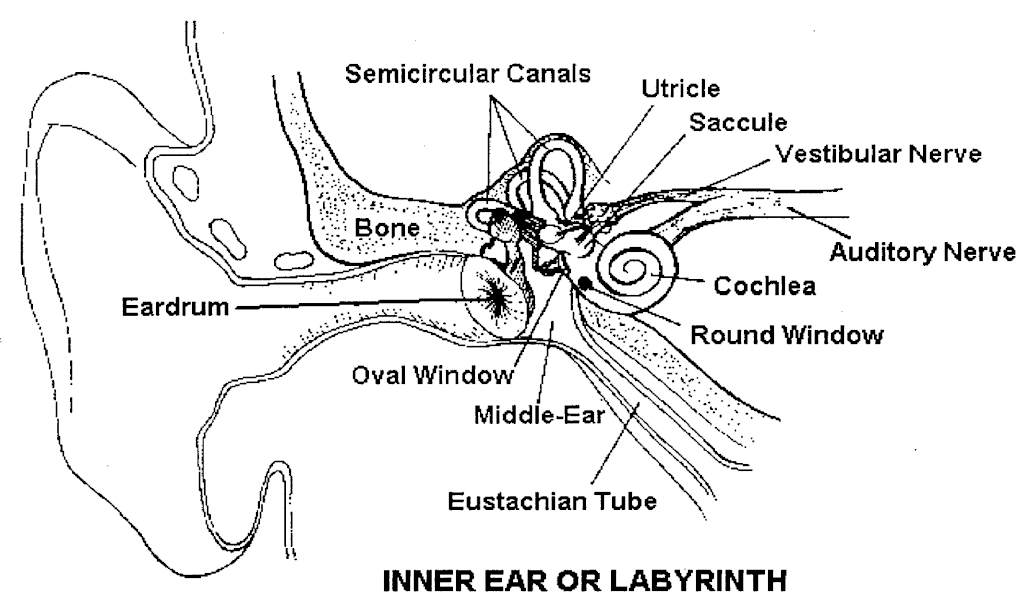
\includegraphics[width=\textwidth]{content/2_related_work/img/VestibularSystem[LaViola2000]}
    \caption{The components of the vestibular system~\cite{LaViola2000}.}
    \label{fig:vestibular-system}
\end{figure}
Important for the sensory conflict theory are visual perception and the vestibular system, shown in
Figure~\ref{fig:vestibular-system}.
The vestibular system consist of the Semicircular Canals to sense angular momentum, and the Utricle and Saccule to
sense linear momentum.
Together, the system functions to compensate for movement, stabilize vision, maintain head posture, and maintain
balance~\cite{Walker2014}.
In virtual environments, the sensory mismatch is usually between the visual system receiving optical flow patterns
characteristic of self motion, while the vestibular system does not perceive these changes in motion.
This sensory conflict lies at the root of simulator sickness and was identified early on, when Barrett and
Thornton~\cite{Barrett1968} noticed that subjects showed simulator sickness symptoms caused by conflict between the
visual presentation of motion and the lack of corresponding vestibular sensation in their fixed-base simulators.
Barrett and Thornton also noticed, that subjects only showed sickness symptoms when the simulator was in a
perspective similar to driving a car, but showed no symptoms when viewing the car from outside, similar to driving a
remote controlled car, as well as passengers showing more severe symptoms than drivers, indicating
that involvement in motion is a factor in the occurrence of simulator sickness~\cite{Tiiro2018,Barrett1968}.

The sensory conflict theory is the most popular theory to explain cybersickness, because it has a steadily growing
amount of studies supporting it, and the theory is intuitive to understand~\cite{Rebenitsch2016,Tiiro2018}.
However, the theory has been criticised by several studies, because sensory conflict theory only states that sickness
is preceded by a sensory conflict, but is unable to predict when cybersickness will occur, or how severe
sickness symptoms will be~\cite{LaViola2000,Rebenitsch2016,Kolasinski1995}.


\subsection{Postural instability theory}\label{subsec:postural-instability-theory}

Another theory for cybersickness symptoms is the postural instability theory proposed by Riccio and Stoffregen~\cite{Riccio1991}.
They found that motion sickness is preceded by periods of postural instability, where small uncontrolled movements and
changes in the subjects centre of gravity occur, and the subject's ability to maintain postural stability is
hindered~\cite{Riccio1991,Clifton2020}.
Stoffregen and Smart~\cite{Stoffregen1998} translated the theory into three predictions:
\begin{itemize}
    \item Experiences of motion sickness are always preceded by increases in postural instability.
    \item Experiences of motion sickness persist until postural stability is restored.
    \item People who are more naturally unstable are more likely to become motion sick during provocative simulation.
\end{itemize}
These predictions have been solidified and are supported by numerous studies on visually induced motion
sickness~\cite{Clifton2020}.
Chardonnet, Mirzaei, and Merienne~\cite{Chardonnet2015}, as well as other studies propose to use the changes in 
range, variance, and frequency of the subject's centre of gravity as a measurement of postural sway.
Based on the accessibility of devices to measure individual's centre of gravity, those measurements have found
increasing popularity in studies to objectively measure subject's postural stability and indicate the potential onset
of cybersickness symptoms~\cite{Lim2020}.
\begin{figure}[h]
    \centering
    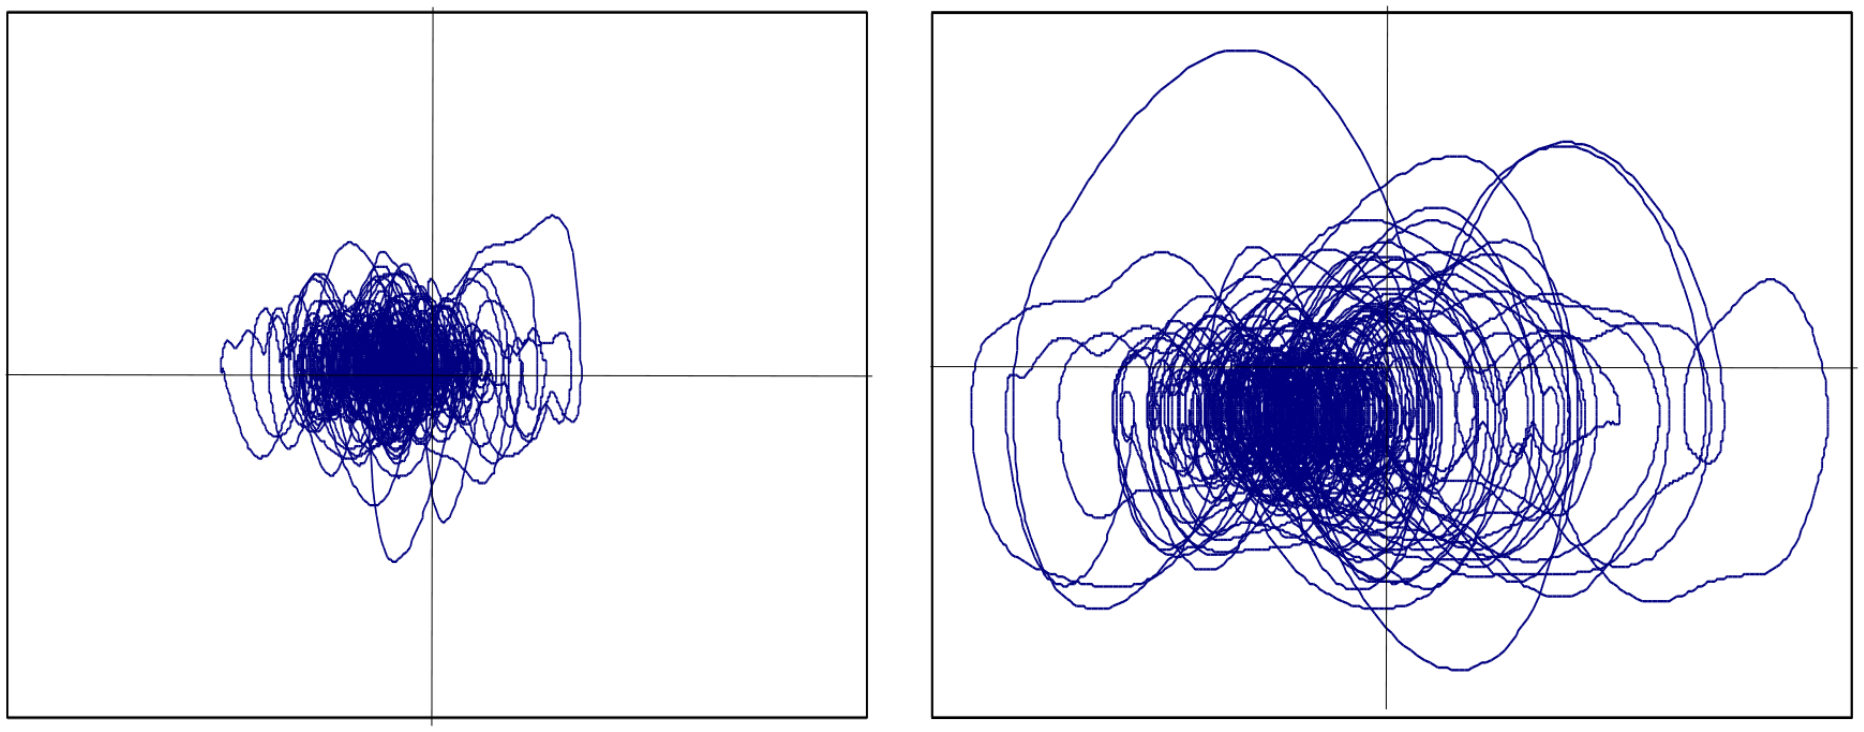
\includegraphics[width=\textwidth]{content/2_related_work/img/PosturalStability[Smart2013]}
    \caption{Comparison of phase portraits (position (in cm) vs. velocity (in cm/s)) for well (left) and sick (right)
        subjects in a dataset measuring postural stability~\cite{Smart2013}.}
    \label{fig:postural-instability-sample}
\end{figure}
A comparison between the natural postural sway of a subject compared to the postural sway when experiencing motion
sickness is shown in Figure~\ref{fig:postural-instability-sample}.
\begin{figure}[h]
    \centering
    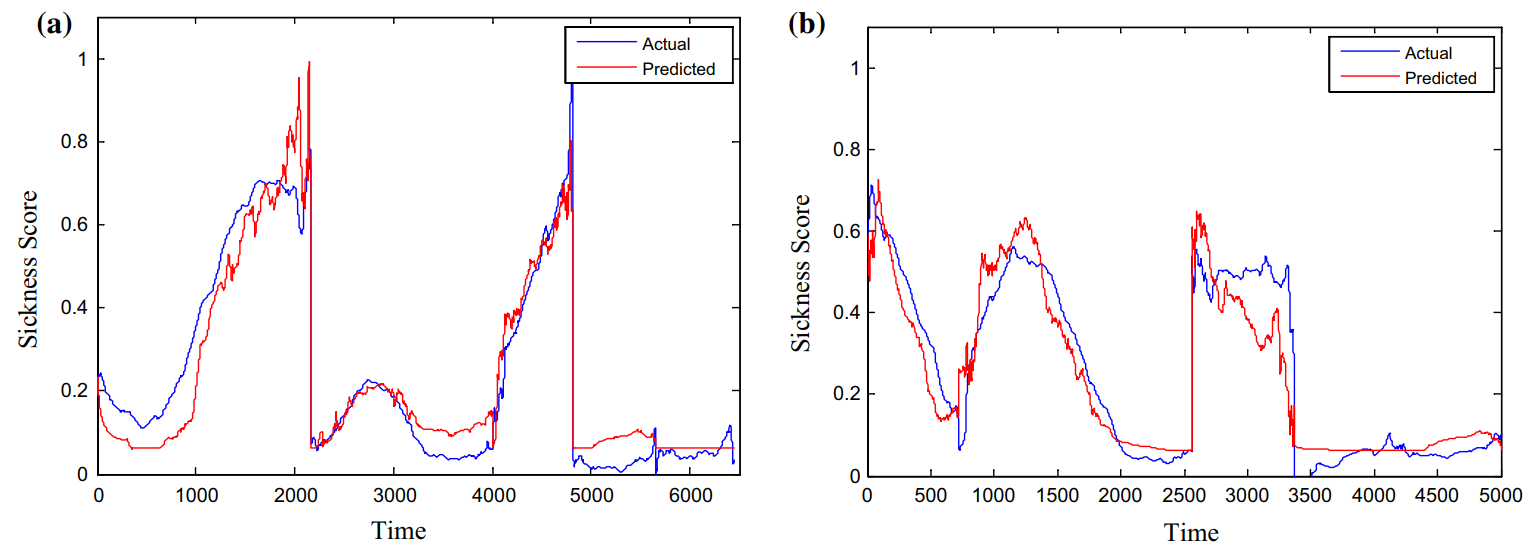
\includegraphics[width=\textwidth]{content/2_related_work/img/PosturalStabilitySicknessPrediction[Lim2020]}
    \caption{Actual sickness (blue) and predicted sickness (red) of (a) training and (b) testing set produced by the
    prediction algorithm by Lim et al.~\cite{Lim2020}.}
    \label{fig:sickness-prediction-algorithm}
\end{figure}
The recent study by Lim et al.~\cite{Lim2020} successfully used postural stability measurements to train an algorithm
to predict VR content's potential to induce cybersickness, as shown in Figure~\ref{fig:sickness-prediction-algorithm},
based on the postural instability theory.


\subsection{Other theories}\label{subsec:other-theories}

\subsubsection{Rest frame theory}
Similar to sensory conflict theory, the rest frame theory argues that a mismatch in sensed gravitation and perceived
up-direction is the cause for sickness symptoms~\cite{Rebenitsch2016}.
\begin{figure}[h]
    \centering
    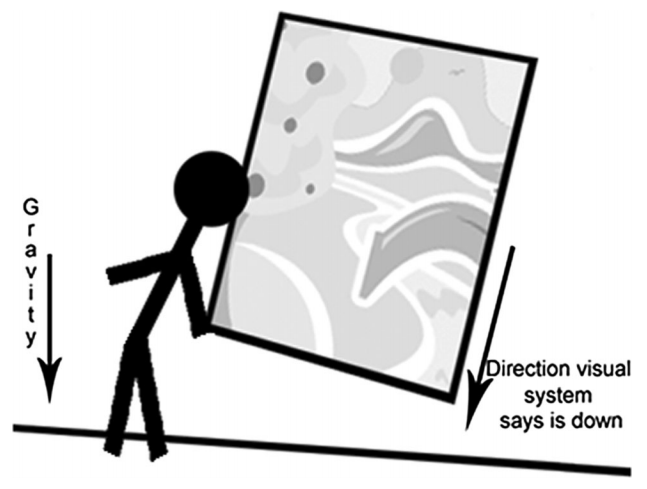
\includegraphics[width=\textwidth/2]{content/2_related_work/img/SensoryMismatchRestFrame[Rebenitsch2016]}
    \caption{Example of sensory mismatch according to rest frame theory~\cite{Rebenitsch2016}.}
    \label{fig:sensory-mismatch-example}
\end{figure}
The rest frame theory also shows similarities to the postural instability theory, as the discrepancy between perceived
up-direction and gravity leads to postural instability and following sickness symptoms~\cite{Rebenitsch2016}.
An example of this sensory mismatch, and resulting postural instability is shown in
Figure~\ref{fig:sensory-mismatch-example}.
The theory also supports the postural instability theory in situations where postural control is lessened, such as in
seated positions where the individual's posture is stabilized.
Several studies like Chang et al.~\cite{Chang2013}, and Duh, Parker, and Furness~\cite{Duh2001b} found, that
superimposing some form of static frame of reference into the virtual environment significantly improves postural
stability and reduces cybersickness symptoms.


\subsubsection{Vergence-accommodation conflict theory}\label{subsubsec:vergence-accommodation-conflict-theory}

Another theory to explain cybersickness symptoms, especially oculomotor symptoms, is the \mbox{vergence-accommodation}
conflict theory.
\begin{figure}[h]
    \centering
    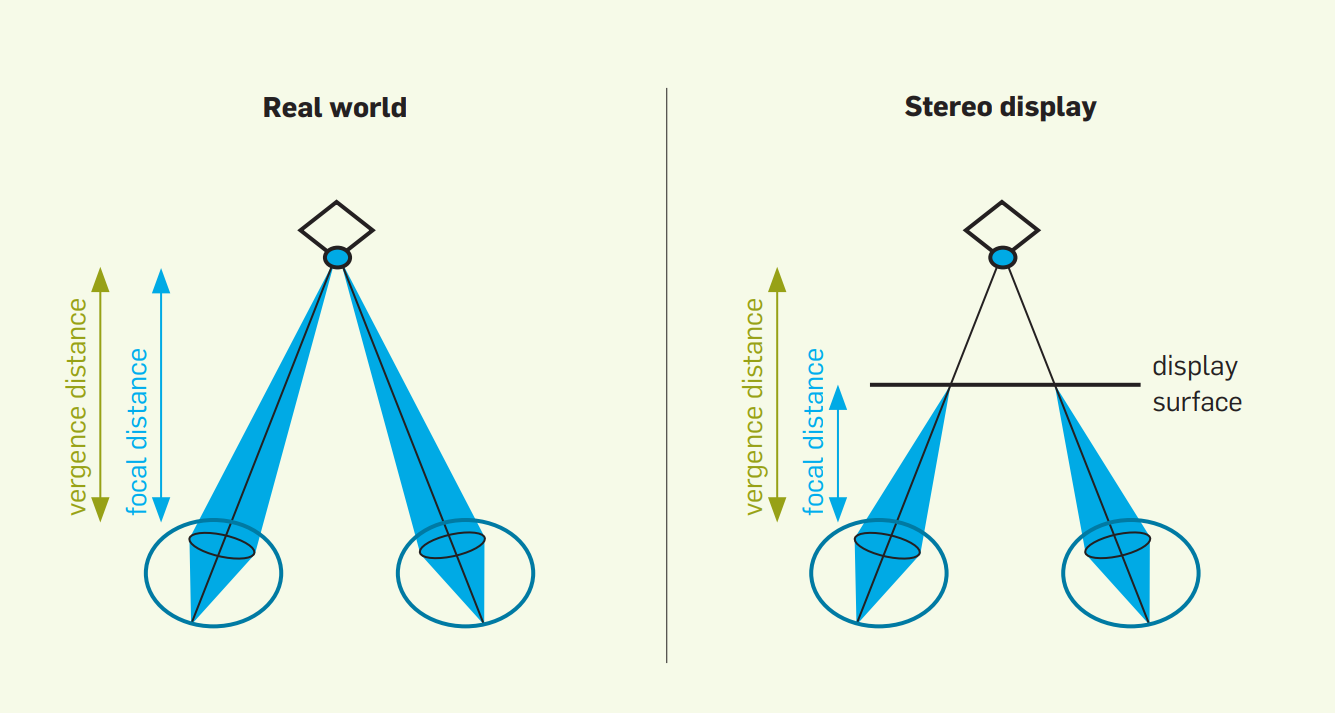
\includegraphics[width=\textwidth/2]{content/2_related_work/img/VergenceAccommodation[Kroeker2010]}
    \caption{Difference between vergence and accomodation distance in the real world (left) and stereoscopic displays
        (right)~\cite{Kroeker2010}.}
    \label{fig:vergence-accommodation-differences}
\end{figure}
Vergence is the simultaneous lateral movement of the eyes when an individual's visual system is adjusting to objects
at different distances~\cite{Kim2014}.
Accommodation is the process of adjusting both eye's focal lengths, focusing on the perceived
object~\cite{Rebenitsch2016}.
In virtual environments, especially in head-mounted displays, images are presented at a fixed screen depth.
This leads to conflict with real life expectations, as vergence and accommodation do not occur naturally at
different distances like in stereoscopic displays~\cite{Saredakis2020}, as shown in
Figure~\ref{fig:vergence-accommodation-differences}.
Kim, Kane, and Banks~\cite{Kim2014} noted that content with high levels of stimulation usually contain more changes
in stimulus distance, and therefore variance of stimulus distance, and level of visual stimulation both increase visual
discomfort and eye strain.


\section{Methods of measurement}\label{sec:methods-of-measurement}

Due to the polysymptomatic and polygenic nature of cybersickness, measurements of cybersickness can prove
difficult, as there is a variety of mostly internal, nonobservable, and subjective symptoms~\cite{McCauley1992}.
Additionally, there can be large individual differences in symptom profiles and susceptibilty, and most symptoms
develop over time and can occur even after the exposure to virtual environments~\cite{McCauley1992}.
Historically, the use of questionnaires is the most popular method of recording occurrences of
cybersickness~\cite{Rebenitsch2016,Saredakis2020}.
The most widely used questionnaire is the Simulator Sickness Questionnaire (SSQ), developed by Kennedy, Lane, Berbaum,
and Lilienthal~\cite{Kennedy1993}.
Recently, several studies have tried refining the SSQ to adapt it for the assessment of virtual reality and
head-mounted displays, resulting in the Virtual Reality Symptom Questionnaire (VRSQ) by Ames, Wolffsohn, and
McBrien~\cite{Ames2005}, and the CyberSickness Questionnaire (CSQ) by Stone III~\cite{Stone2017}.
Another popular questionnaire is the broader formulated Motion Sickness Assessment Questionnaire (MSAQ) by Gianaros,
Muth, Mordkoff, Levine, and Stern~\cite{Gianaros2001}, designed to assess visually-induced motion sickness symptoms
regardless of stimulus context.
In addition to the extensive post-session questionnaires, single item questionnaires like the Fast Motion Sickness
Scale (FMS) by Keshavarz and Hecht~\cite{Keshavarz2011} that are polled in regular intervals during the virtual
environment exposure have gained popularity in cybersickness studies.
Because of the subjective nature of questionnaires, these methods of quantifying cybersickness symptoms have been
criticised and several methods of objective measurement have been researched.
Kim et al.~\cite{Kim2005} studied the changes in sixteen different electrophysiological signals and found several
measurements with a significant positive or negative correlation.
However, these measurements require special equipment that may be unavailable or unintuitive, leading to a low
adoption rate among studies related to cybersickness symptoms and detection.
A more easily accessible method of objective measurement has been measuring the postural stability of individuals
exposed to virtual environments and use the changes in the centre of gravity (CoG) as an indicator for cybersickness
symptoms~\cite{Lim2020}.


\subsection{Subjective Measurements}\label{subsec:subjective-measurements}

\subsubsection{Simulator Sickness Questionnaire}\label{subsubsec:simulator-sickness-questionnaire}

The Simulator Sickness Questionnaire developed by Kennedy, Lane, Berbaum, and Lilienthal~\cite{Kennedy1993} is,
despite being developed in 1993, still one of the most popular methods to measure cybersickness
symptoms~\cite{Saredakis2020}.
Kennedy et al.\ based their developments on the Pensacola Motion Sickness Questionnaire (MSQ), where they identified
several deficiencies that could be improved:
\begin{itemize}
    \item to provide a more valid index of overall simulator sickness severity as distinguished from motion sickness;
    \item to provide subscale scores that are more diagnostic of the locus of simulator sickness in a particular
    simulator for which overall severity was shown to be a problem;
    \item to provide a scoring approach to make monitoring and cumulative tracking relatively straightforward.
\end{itemize}
As part of the last objective, they sought to eliminate the configural approach of the MSQ allowing to automate the
administration and scoring of results.
Additionally, the studies involving the MSQ used differences between post- and pre-exposure scores as their main
indicator, and a pre-exposure checklist where subjects are asked whether they were in other than their "usual state 
of fitness".
Kennedy et al.\ removed both, the two-step approach, and the pre-exposure checklist in an effort to streamline the
administration and scoring process, noting that the SSQ is "intended only for application to post-exposure symptoms,
with the further precondition that a screening of "unhealthy" subjects is required [before exposure]"~\cite[p.
207]{Kennedy1993}.
To tailor the questionnaire to better fit simulator exposure and its sickness symptoms, Kennedy et al.\ eliminated
symptoms that might give misleading indication, were selected too infrequently, or showed no change in frequency or
severity.
Additionally, they sorted the remaining symptoms into separate clusters labeled "Oculomotor" (SSQ-O),
"Disorientation" (SSQ-D), and "Nausea" (SSQ-N).
The distinction allowed to apply a subscale to each cluster, reflecting the impact of simulator exposure on a
different "target system" in the subject.
It also simplified the process of determining where and in what way a simulator may cause problematic
symptoms.
\begin{center}
    \begin{tabular}{ l c c c}
        \toprule
        \textbf{ } & \textbf{ } & \textbf{Weight} & \textbf{ } \\
        \textbf{SSQ Symptom} & \textbf{$N$} & \textbf{$O$} & \textbf{$D$} \\
        \midrule
        General discomfort          & 1 & 1 &   \\
        Fatigue                     &   & 1 &   \\
        Headache                    &   & 1 &   \\
        Eyestrain                   &   & 1 &   \\
        Difficulty focusing         &   & 1 & 1 \\
        Increased salivation        & 1 &   &   \\
        Sweating                    & 1 &   &   \\
        Nausea                      & 1 &   & 1 \\
        Difficulty concentrating    & 1 & 1 &   \\
        Fullness of head            &   &   & 1 \\
        Blurred vision              &   & 1 & 1 \\
        Dizzy (eyes open)           &   &   & 1 \\
        Dizzy (eyes closed)         &   &   & 1 \\
        Vertigo                     &   &   & 1 \\
        Stomach awareness           & 1 &   &   \\
        Burping                     & 1 &   &   \\
        \\
        Total                       & [1] & [2] & [3] \\
        \\
        Score & & & \\
        $N = [1] \times 9.54$ & & & \\
        $O = [2] \times 7.58$ & & & \\
        $D = [3] \times 13.92$ & & & \\
        $TS = [1] + [2] + [3] \times 3.74$ & & & \\
        \bottomrule
    \end{tabular}
    \captionof{table}{SSQ Symptoms and Scoring according to Kennedy et al.~\cite{Kennedy1993}.}
    \label{tab:ssq-scoring}
\end{center}
Table~\ref{tab:ssq-scoring} shows the remaining symptoms and their clustering, as well as the method of scoring the
SSQ as derived by Kennedy et al.
The SSQ symptoms are rated on a four-point scale from 0 to 3, then multiplied by either 1 or 0 (omitted in the table)
according to the weight section of table~\ref{tab:ssq-scoring}, and finally summed up in each column.
The total and subscale scores are then calculated using the formulas in the "Score" section of
table~\ref{tab:ssq-scoring}.
Kennedy et al.\ also mention the possibility to further refine the questionnaire by:
\begin{itemize}
    \item splitting the "Oculomotor" cluster into the disturbance of visual processing (blurred vision, difficulty
    focusing) and the symptoms caused by the disturbance (headache, eyestrain);
    \item splitting the "Nausea" cluster into premonitory signs (increased salivation, burping) and advanced stages
    of nausea (nausea, sweating);
\end{itemize}
As well as moving some symptoms into a "tired and hungry" cluster, believed to be an artifact created by the time
spent during the exposure.
However, Kennedy et al.\ state that there are not enough simulator-relevant symptoms to provide adequate reliability
for smaller clusters, and recommend using the three cluster solution.
Despite the general adoption of the SSQ, there are several problems, especially for the assessment of
cybersickness symptoms in virtual environments, that Kennedy et al.\ recognize in their study.
\begin{center}
    \begin{tabular}{ l l c c c c}
        \toprule
         & & & \textbf{SSQ} & \textbf{Scale M} & \\
        \textbf{Simulator} & \textbf{Aircraft} & \textbf{$N$} & \textbf{$O$} & \textbf{$D$} & \textbf{$TS$*} \\
        \midrule
        2F64C & SH-3   & 14.7 & 20.0 & 12.4 & 18.8 \\
        2F120 & CH-53E & 7.5  & 10.5 & 7.4  & 10.0 \\
        2F121 & CH-53D & 7.2  & 7.2  & 4.0  & 7.5  \\
        2F110 & E-2C   & 7.1  & 13.1 & 6.8  & 10.3 \\
        2E7   & F/A-18 & 6.1  & 5.1  & 6.2  & 6.8  \\
        2F117 & CH-46E & 5.4  & 7.8  & 4.5  & 7.0  \\
        2F87F & P-3C   & 4.5  & 15.2 & 4.3  & 10.5 \\
        2F132 & F/A-18 & 2.7  & 6.1  & 0.6  & 4.2  \\
        2F112 & F-14   & 1.7  & 1.8  & 0.0  & 1.5  \\
              &        &      &      &      &      \\
        M     &        & 7.7  & 10.6 & 6.4  & 9.8  \\
        SD    &        & 15.0 & 15.0 & 15.0 & 15.0 \\
        \bottomrule
        * Total Severity & & & & & \\
    \end{tabular}
    \captionof{table}{SSQ Scale Means by Simulator for the Calibration Sample according to Kennedy et al
    .~\cite{Kennedy1993}.}
    \label{tab:ssq-calibration}
\end{center}
The weights for the scoring functions are derived from 1119 pairs of MSQs collected from 9 simulator sites
shown in table~\ref{tab:ssq-calibration} as a calibration sample.
Therefore, the modal position on the Symptoms or the intermediate sums is no indication for symptomatology with
respect to simulator sickness across simulators in general, as the zero point contains between 40\% and 75\% of the
observations in the calibration dataset.
This also means, the sensitivity is at the upper extremes of the symptomatology range, and the scores should be
compared to the calibration set, in table~\ref{tab:ssq-calibration}, instead of
interpreted on their own~\cite{Kennedy1993}.
Kennedy et al.\ conclude that the results should not be used to distinguish among simulators without problems, but
identify and discriminate problem simulators from those without problems.
Other, more recent studies, like Sevinc and Berkman~\cite{Sevinc2020}, and Rebenitsch and Owen~\cite{Rebenitsch2016},
criticise the usage of the Simulator Sickness Questionnaire because of its complex structure, and development
process, as it involves only a sample of highly trained professionals, and a small amount of simulator experiments,
which both do not comply with the modern day HMD-based virtual environments, and diverse applications
and users~\cite{Sevinc2020}.

\subsubsection{Virtual Reality Symptom Questionnaire}\label{subsubsec:virtual-reality-symptom-questionnaire}

Recent studies like Ames, Wolffsohn, and McBrien~\cite{Ames2005} tried to develop a questionnaire based on the MSQ
and SSQ specifically for the assessment of cybersickness symptoms.
Ames et al.\ note that existing methods like the SSQ do not properly address the ocular symptoms that
contribute to cybersickness symptoms in virtual environments.
Examining existing virtual reality research, they identified 23 symptoms split into two clusters, 12 non-ocular, and
11 ocular symptoms.
Ames et al.\ also decided to expand the symptom response scale to seven options sorted into four
labels: "none" (0), "slight" (1, 2), "moderate" (3, 4), and "severe" (5, 6).
In the development study, they exposed 16 subjects to a stereoscopic video played on a
head-mounted display, and recorded the occurring symptoms with the developed VRSQ in two-minute
intervals immediately after the exposure for a total of six post-exposure examinations.
From the results, they identified 13 symptoms with high item-total correlations, that remain in the final
questionnaire.
While, the "nausea" symptom did not meet the correlation criteria, it was retained for research that might involve
more "dynamic imagery".
However, similar studies, like Stone III~\cite{Stone2017}, criticise the validity of the VRSQ to evaluate
cybersickness, as Ames et al.\ only used video input on a head-mounded display, without any user interaction or input
method, resulting in visual stimulus only, similar to existing studies on visually induced motion sickness, but not
explicitly virtual reality sickness symptoms.
Additionally, Stone III notes concerns about the validity of the psychometric evaluation, and the small sample size
used in the development study.
Davis, Nesbitt, and Nalivaiko~\cite{Davis2014} also note the lack of published studies using the VRSQ as a method to
evaluate cybersickness symptoms in their review on cybersickness literature, while Rebenitsch et al
.~\cite{Rebenitsch2016} do not mention the VRSQ at all.

\subsubsection{CyberSickness Questionnaire}\label{subsubsec:cybersickness-questionnaire}

In his study criticising the VRSQ and SSQ, Stone III~\cite{Stone2017} also proposes an alternative solution to
measure cybersickness symptoms, the CyberSickness Questionnaire (CSQ).
Similar to the method Kennedy et al.\ \cite{Kennedy1993} used to refine the SSQ from the MSQ, they reinterpreted the
results of the SSQ in a cybersickness context.
For this, Stone III selected the symptoms clearly indicating cybersickness:
\begin{itemize}
    \item headache
    \item eyestrain
    \item nausea
    \item blurred vision
    \item dizzy (eyes open)
    \item dizzy (eyes closed)
    \item vertigo
    \item difficulty focusing
    \item fullness of head
\end{itemize}
Additionally, they decided to amalgamate "Severe" and "Moderate" responses from the SSQ\@.
Stone III found a two factor solution by separating the Symptoms into two clusters: "Dizziness" and
"Difficulty focusing".
They also note that the SSQ can still be used to record post-exposure symptoms, while the
scoring can be done using the developed CSQ approach by following these steps:
\begin{enumerate}
    \item Administer the SSQ after the exposure to virtual environments.
    \item Remove the unneccesary symptom items from the collected data.
    \item Combine "Moderate" and "Severe" options for each symptom item, resulting in responses "None" (0), "Slight"
    (1), and "Moderate" (2).
    \item Compute the CSQ factors, similar to the SSQ, by multiplying each symptom item with the weight shown in
    table~\ref{tab:csq-scoring} and adding up the items to form the final scores.
\end{enumerate}
\begin{center}
    \begin{tabular}{ l c c}
        \toprule
        \textbf{} & \textbf{Dizziness} & \textbf{Difficulty focusing} \\
        \midrule
        Headache                & $.50$ & $.$   \\
        Eyestrain               & $.$   & $.58$ \\
        Difficulty focusing     & $.$   & $.89$ \\
        Nausea                  & $.84$ & $.$   \\
        Fullness of head        & $.$   & $.55$ \\
        Blurred vision          & $.$   & $.81$ \\
        Dizziness (eyes open)   & $.89$ & $.$   \\
        Dizziness (eyes closed) & $.99$ & $.$   \\
        Vertigo                 & $.54$ & $.$   \\
        \bottomrule
    \end{tabular}
    \captionof{table}{CSQ nine-item, two-factor model for scoring, according to Stone III~\cite{Stone2017}}
    \label{tab:csq-scoring}
\end{center}
Stone III notes that preliminary evidence, and the comparison of CSQ scores with other established visually-induced
motion sickness scoring methods support the validity of the resulting CyberSickness Questionnaire.
However, they note based on the CSQ scores of their study, 57\% of the 202 participants reported no dizziness and 40\%
reported no difficulty focusing, which implies cybersickness was very low, and the study was not focused
explicitly on inducing cybersickness symptoms.
The review of questionnaires by Sevinc et al.~\cite{Sevinc2020} has tested and approved the validity of the CSQ and
concludes that it is a more accurate method of measuring cybersickness symptoms than the SSQ, as it was developed
with a lager sample size and specifically based on the use of virtual reality applications to induce sickness symptoms.

\subsubsection{Motion Sickness Assessment Questionnaire}\label{subsubsec:motion-sickness-assessment-questionnaire}

Gianaros, Muth, Mordkoff, Levine, and Stern~\cite{Gianaros2001} developed the Motion Sickness Assessment
Questionnaire (MSAQ) with the goal to assess motion sickness across a broad range of contexts.
Similar to other studies developing questionnaires, Gianaros et al.\ recognized the multi-dimensionality of motion
sickness symptoms.
However, they felt sopite-related symptoms, like drowsiness, yawning, and disengagement from the environment, were
underrepresented in existing questionnaires~\cite{Gianaros2001,Graybiel1976}.
Including sopite-related symptoms, Gianaros et al.\ identified four dimensions of motion sickness:
\begin{itemize}
    \item gastrointernal symptoms, like sickness, queasiness, or nausea;
    \item central symptoms, like dizziness, disorientation, lightheadedness, or blurred vision;
    \item peripheral symptoms, like being sweaty, clammy, or hot, or cold sweat;
    \item sopite symptoms, like being annoyed, tired, fatigued, or uneasy.
\end{itemize}
Similar to the SSQ, they designed the MSAQ to be used both, for overall motion sickness scores, and assessment of 
distinct dimensions via subscale scores.
\begin{center}
    \begin{tabular}{l c c c c}
        \toprule
        \textbf{Symptom Item} & \textbf{Gastrointestinal} & \textbf{Central} & \textbf{Peripheral} & \textbf{Sopite} \\
        \midrule
        I felt sick to my stomach  & $.36$ & $.$   & $.$   & $.$   \\
        I felt faint-like          & $.$   & $.45$ & $.$   & $.$   \\
        I felt annoyed/irritated   & $.$   & $.$   & $.$   & $.36$ \\
        I felt sweaty              & $.$   & $.$   & $.27$ & $.$   \\
        I felt queasy              & $.36$ & $.$   & $.$   & $.$   \\
        I felt lightheaded         & $.$   & $.45$ & $.$   & $.$   \\
        I felt drowsy              & $.$   & $.$   & $.$   & $.36$ \\
        I felt clammy/cold sweat   & $.$   & $.$   & $.27$ & $.$   \\
        I felt disoriented         & $.$   & $.45$ & $.$   & $.$   \\
        I felt tired/fatigued      & $.$   & $.$   & $.$   & $.36$ \\
        I felt nauseated           & $.36$ & $.$   & $.$   & $.$   \\
        I felt hot/warm            & $.$   & $.$   & $.27$ & $.$   \\
        I felt dizzy               & $.$   & $.45$ & $.$   & $.$   \\
        I felt like I was spinning & $.$   & $.45$ & $.$   & $.$   \\
        I felt as if I may vomit   & $.36$ & $.$   & $.$   & $.$   \\
        I felt uneasy              & $.$   & $.$   & $.$   & $.36$ \\
        \bottomrule
    \end{tabular}
    \captionof{table}{Symptom items and subscale groups, according to Gianaros et al.~\cite{Gianaros2001}}
    \label{tab:msaq-questions}
\end{center}
The Questionnaire consists of between 16 and 20 symptom questions, with the original 16 questions shown in
table~\ref{tab:msaq-questions}~\cite{Gianaros2001,Sevinc2020}.
Each symptom question is rated on a nine-point scale from 1 (Not at all) to 9 (Severly).
The subscale scores are the sum of the weighted symptom items, multiplied by the weights in the respective columns, and
the total motion sickness score is obtained by the following formula, according to Gianaros et al.:
\begin{itemize}
    \item Overall Motion Sickness Score $= ($ sum of all symptom items (without weights) $) \times 1.44$
\end{itemize}
While, Gianaros et al.\ note that the generated symptoms during their study may stem from a relatively narrow range
of motion sickness contexts, they offer the possibility to modify the questionnaire to more accurately reflect the
multiple dimensions of motion sickness across different motion environments.
Although the development process of the questionnaire was based on visually-induced motion sickness using optokinetic
drums and not virtual reality environments, Sevinc et al.~\cite{Sevinc2020} note in their review on cybersickness
that the Motion Sickness Assessment Questionnaire was used in several virtual reality and simulator studies in the
recent years.
Lastly, Gianaros et al.\ argue that their questionnaire supplies valid descriptors of motion sickness in and for
general population, since the symptom items were generated independently by non-experts during the early phases of
their study.

\subsubsection{Fast Motion Sickness Scale}\label{subsubsec:fast-motion-sickness-scale}

In contrast to the multi-dimensional questionnaires, Keshavarz and Hecht~\cite{Keshavarz2011} proposed and validated
a single-item questionnaire that can be administered during stimulus presentation.
This allows for simple and continuous gathering of motion sickness data during the presentation.
The FMS consists of a verbal rating every minute on a 20-point scale between 0 (no sickness) and 20 (frank sickness),
and primarily measures the two cardinal symptoms in motion sickness: nausea, and general
discomfort~\cite{Keshavarz2011}.
Keshavarz and Hecht explain, they use a 20-point scale to better differentiate among lower
degrees of motion sickness symptoms and capture different states of both well-being and sickness.
They argue the extended scale also helps participants to express their feelings and experience more precisely.
Conversely, Keshavarz and Hecht also note the questionnaire's indifference to the physiological correllates or root
causes of motion sickness, and participants are unable to differentiate between nausea and other precursor symptoms
in their answers.
In their defense, they argue the Fast Motion Sickness Scale is only designed to quantify the subjective impressions
of nausea and general discomfort related to motion sickness, without addressing the underlying symptoms or causes.
\begin{figure}[h]
    \centering
    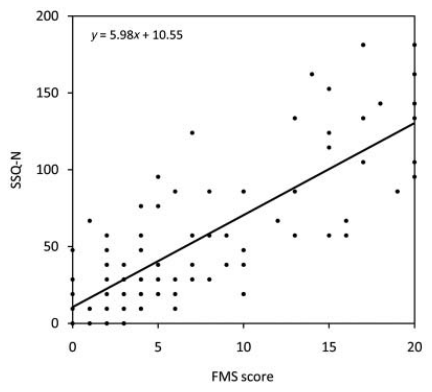
\includegraphics[width=\textwidth/2]{content/2_related_work/img/FMStoSSQcorrelation[Keshavarz2011]}
    \caption{Scatter plot showing the distribution of peak FMS score and SSQ-N subscore for all participants of the
    study by Keshavarz and Hecht~\cite{Keshavarz2011}.}
    \label{fig:fms-ssq-correlation}
\end{figure}
Their validation study showed high correlation between the peak scores of the FMS and the Nausea subscale score of
the Simulator Sickness questionnaire (SSQ-N), as shown in figure~\ref{fig:fms-ssq-correlation}.
Additionally, Rebenitsch and Owen~\cite{Rebenitsch2016} conclude that one-item rating scales are acceptable to
monitor motion sickness symptoms, even though they are not as sensitive or thorough as the multi-dimensional, longer
Questionnaires.
Sevinc and Berkman~\cite{Sevinc2020} also mention a rise in single-item assessment methods, but note that the FMS is
the only version that has been psychometrically evaluated.


\subsection{Objective Measurements}\label{subsec:objective-measurements}

In contrast to the subjective measurements that have been employed in most studies on cybersickness, several studies
have tried linking physiological measurements to the occurrence of cybersickness symptoms in individuals.
Finding reliable physiological cybersickness indicators potentially allows monitoring symptoms without interrupting
the virtual reality exposure through frequent polling of the subject, as used in the FMS, while still generating a
continuous measurement stream to examine symptom development and causes over the duration of the virtual environment
exposure~\cite{Rebenitsch2016}.
One of the broadest studies regarding objective measurements of cybersickness symptoms is the study by
Kim et al.~\cite{Kim2005}, where they collected and tested 16 electrophysiological signals that were used in other
studies as measurements of sickness symptoms in order to find significant correlations indicating a reliable,
objective method measuring cybersickness.
The signals collected before, during, and after the exposure included the following items, which showed a significant
correlation to reported sickness in previous studies:
\begin{itemize}
    \item heart period
    \item respiratory sinus arrhythmia
    \item respiration rate
    \item eyeblink rate
    \item fingertip pulse volume
    \item fingertip temperature
    \item skin conductance
    \item gastric tachyarrhythmia (arrhythmic disruptions of the gastric musculature, often resulting in an upset
    stomach or uneasy feeling)
    \item electroencephalogram (EEG) power spectrum
\end{itemize}
Kim et al.\ used a quite provocative stimulus to test the physiological signals, as 45 out of the 57 subjects
experienced cybersickness symptom during the 9.5 minutes of exposure to virtual environments and subjects reported
cybersickness an average of five times during the exposure.
They also employed a 33-item pre-immersion, and a 49-item post immersion questionnaire to link to better link their
electrophysiological findings to the self-reported levels of cybersickness symptoms experienced.
The questionnaires were compilations of different popular cyber- and motion sickness and susceptibility questionnaires
including the Simulator Sickness Questionnaire.
Kim et al.\ found significant correlations, especially between SSQ scores and gastric tachyarrhythmia, eyeblink rate,
respiration rate, respiration sinus arrhythmia, and heart period.
They found, gastric tachyarrhythmia, skin conductance, respiratory sinus arrhythmia, and relative delta power at F3
and T3 electrode locations of the EEG were significantly higher than the previous recorded baseline.
They also found, heart period, fingertip skin temperature, fingertip pulse volume maximum amplitude, and relative
beta power at F3 and T3 electrode locations were significantly decreased compared to the recorded baseline.
Kim et al.\ suggest that due to the correlation between gastric tachyarrhythmia and cybersickness, the autonomic
nervous system may play a bigger part in the occurrence of cybersickness than previously assumed.
Similar to this study, Roberts and Gallimore~\cite{Roberts2005} found electrogastrogram (EGG) measurements, to detect
gastric tachyarrhythmia, to be a strong indicator of virtual reality exposure and cybersickness symptoms.
Other studies have also used electrocardiogram (ECG) and blood pressure measurements to indicate cybersickness, as 
they found the heart beat becomes stronger, and the blood flow shows lower turbulence during exposure to virtual
environments~\cite{Kiryu2007, Watanabe2008}.

Davis et al.~\cite{Davis2014} note that one detractor to widespread use of physiological measurements may be the
costly hardware and difficulty to analyse the results.
A middle ground has been presented in several studies using measurements of postural stability as an objective, low
cost, and continuous indicator of cybersickness symptoms~\cite{Rebenitsch2016}.
However, Rebenitsch et al.~\cite{Rebenitsch2016} also note that postural sway measurements in many studies are not as
continuous or without the disturbance of the subject as they are often presented, since most measurements require the
subject to enter a specific stance for the measurement.
Most studies use the amplitude, magnitude, and frequency of postural sway to distinguish and predict motion sickness
symptoms, while older studies also examine the time till failure (time until a stance cannot be maintained) or the
stance breaks (number how often the subject fails to maintain a stance) during a specific
timeframe~\cite{Rebenitsch2016}.
Villard, Flanagan, Albanese, and Stoffregen~\cite{Villard2008} and Dong, Stoffregen, and
Yoshida~\cite{Dong2011, Dong2010} both noticed in their studies that subjects who did not experience significant
sickness symptoms had an increased standard deviation of motion during their exposure period, while subjects that
experienced sickness symptoms showed greater variability with smaller average motion compared to the baseline.
Some other studies mentioned similar findings and suggest that subjects may self-adapt to virtual reality exposure by
consciously avoiding head movements when experiencing sickness symptoms~\cite{Rebenitsch2016}.
Another method of low cost, objective measurement of cybersickness is presented by Chardonnet et
al.~\cite{Chardonnet2015}, who found consistent results measuring a subject's centre of gravity (CoG) with a high
correlation to measured SSQ scores.
Lim, Lee, Won, Kala, and Lee~\cite{Lim2020} further extended this measurement, as they proposed to use the VR devices
inertial measurement unit (IMU) to record head dispersion during the exposure period.
They introduced Head Dispersion as a measurement of stability from the following Eq.~\ref{eq:head-dispersion}
\begin{equation}
    \label{eq:head-dispersion}
    Head\ Dispersion = \sqrt{\frac{\sum(roll - \overline{roll})^2 + \sum{(pitch - \overline{pitch})^2}} {n}}
\end{equation}
With the $roll$ and $pitch$ values in degree, and $\overline{roll}$ and $\overline{pitch}$ as the mean values along
the session.
To validate their approach Lim et al.\ compared their IMU sensor data to the centre of gravity sway area measured by an
external sensor as proposed by Chardonnet et al.\ and found high correlation between their measured Head Dispersion
and CoG sway area.
The major advantages of this method are the lack of additional measuring devices needed, and the synchronization
processing, while delivering a continuous indicator of potential sickness symptoms.
However, due to the study's recency, it has not yet seen further adoption or larger sample size studies.


\section{Methods of Mitigation}\label{sec:methods-of-mitigation}

Despite the lack of a definitive cause or widespread adoption of objective measurements to monitor cybersickness
symptoms, several mitigation techniques and best practices have proven effective and have found widespread adpotion
as early as 1992, when McCauley and Sharkey~\cite{McCauley1992} formulated their best practices and recommendations
to prevent and mitigate cybersickness and simulator sickness symptoms:

\textit{Exposure time should be limited until adaption to the VE has occurred}, as some studies found that users
adapt to virtual environments with repeated exposure~\cite{Hill2000}.

\textit{Tasks that require high rates of linear or rotational acceleration should be avoided, or kept brief, until the
individual has fully adapted to the altered environment}, as virtual reality content with high interaction and visual
stimulation tends to lead to more severe experiences of motion sickness~\cite{Saredakis2020}.

\textit{Users of VEs should be considered on an individual basis when determining an adaptation program}.
While this recommendation is focused on adaption programs for simulators, it is also applicable to virtual reality
users, as they show individual differences in cybersickness susceptibility or, for example, preferred locomotion 
method~\cite{Clifton2020}.

\textit{Self-movement through a VE should be at high altitudes above the terrain and/or at lower speeds}, as high
peripharal motion and visual flow are related to cybersickness occurrence and severity~\cite{Buhler2018}.

Additionally, \textit{unusual and extraordinary maneuvers should be avoided in VEs}, as abrupt and counterintuitive
movements can further disorient the user, increasing the risks of cybersickness.

Finally, \textit{users of VE systems should be informed of the possible adverse effects and should be advised to
allow for recovery time after cybertravel before actively engaging in potentially dangerous activities in the real
world, such as driving}, since studies have shown that cybersickness symptoms can occur delayed after the exposure
and have potentially lingering effects~\cite{LaViola2000}.

Apart from these general recommendations, several techniques have found widespread adoption and have shown a positive
impact in mitigating cybersickness symptoms, like the limitation of the Field of View, or the insertion of stable
frames of reference into the virtual scene.


\subsection{Field of View Limitation}\label{subsec:field-of-view-limitation}

The interaction between Field of View (FoV), cybersickness, and the individual's feeling of presence, have been the
subject of many studies, trying to identify the connections and possibly find an optimal solution for the FoV, where
cybersickness symptoms are minimised, while maintaining the feeling of presence as much as possible~\cite{Weech2019}.
Duh et al.~\cite{Duh2001} also found vection to be strongly tied to FoV, as subjects mainly seem to receive
information about vection from their peripheral visual field.
Therefore, a wide FoV causes a greater perception of self-motion, which tends to lead to increased postural
disturbance, and generally resulting in more severe cybersickness symptoms.
Studies like Fernandes and Feiner~\cite{Fernandes2016} recommend to dynamically or at least strategically manipulate
the Field of View in order to reduce visual flow in the peripheral field during periods of high visual flow, reducing
the impact of the resulting vection on cybersickness symptoms.
Duh et al.\ examined the limits of narrow Field of Views and found that, while the experienced motion sickness
increased with higher FoV, there is a significant increase at the 120\textdegree-150\textdegree interval.
Additionally, participants in the study by Lim et al.~\cite{Lim2020} reported "less noticeable" black regions until
the FoV dropped below 60\textdegree.
Lim et al.\ conclude that FoV limitations should be individually adjusted, as users react differently to varying
degrees of FoV limitations, as well as dynamic and fixed FoV limitation.
Finally, they note that, according to their study, dynamic FoV processing and limiting can decrease VR sickness
symptoms by up to 37\%.

    \chapter{Current State/Problems of CosmoScout}\label{ch:current-state/problems-of-cosmoscout}


\section{CosmoScout Concepts}\label{sec:cosmoscout-concepts}
\subsection{SPICE Coordinate Systems}\label{subsec:spice-coordinate-systems}


\section{Problems with free movement}\label{sec:problems-with-free-movement}


\section{Problems with automatic movement}\label{sec:problems-with-automatic-movement}

    \chapter{Implemented Solutions}\label{ch:implemented-solutions}

\section{Floor Grid}\label{sec:floor-grid}

As suggested in the studies examined in section~\ref{subsubsec:stable-reference-frame}, we decided to add a stable
reference frame to help with postural stability.
Especially, we focus on the 6-Degrees-of-Freedom navigation in the interplanetary areas of the Simulation, that
generally lack any sort of fixed reference frame, since movement on a planet surface has the surface and its normal
direction as a strong visual indicator for a reference frame.

The floor grid aims to provide a definitive up-direction that is parallel to the real world's gravity, thereby
improving postural stability and minimizing sensory conflicts.
While superimposing a grid on the floor may significantly reduce the feeling of presence, we accept this effect since
the primary function of CosmoScout VR as a scientific visualization tool is not as dependent on an immersive feeling
as entertainment oriented simulations may be.

Additionally, we also suspect that small changes to the control scheme can be done to further change the interaction
context from an egocentric view within the simulation to a more exocentric "Pseudo AR" approach, where the user
manipulates the surrounding simulation without moving, similar to the Worlds-in-Miniature approach proposed
by Drogemuller et al.~\cite{Drogemuller2020}.

The Hypothesis is that a "Pseudo AR" simulation environment would drastically reduce cybersickness symptoms, as the
sensory conflict between the user inside the simulation and the real world is minimal, and maintaining postural
stability should be easier for the user.
Additionally, the best practices mentioned by McCauley et al.~\cite{McCauley1992}, include that users should be
considered individually as reaction and adaptation to virtual environments are different for each case.
In order to match individual users adaptation progress, as well as different scenarios regarding the hardware setup,
most values and aspects of the grid can be customised through the settings file and almost all of them are also
changeable in the options menu at runtime.

\subsection{Floor Grid Implementation}\label{subsec:floor-grid-implementation}

\begin{figure}[h]
    \centering
    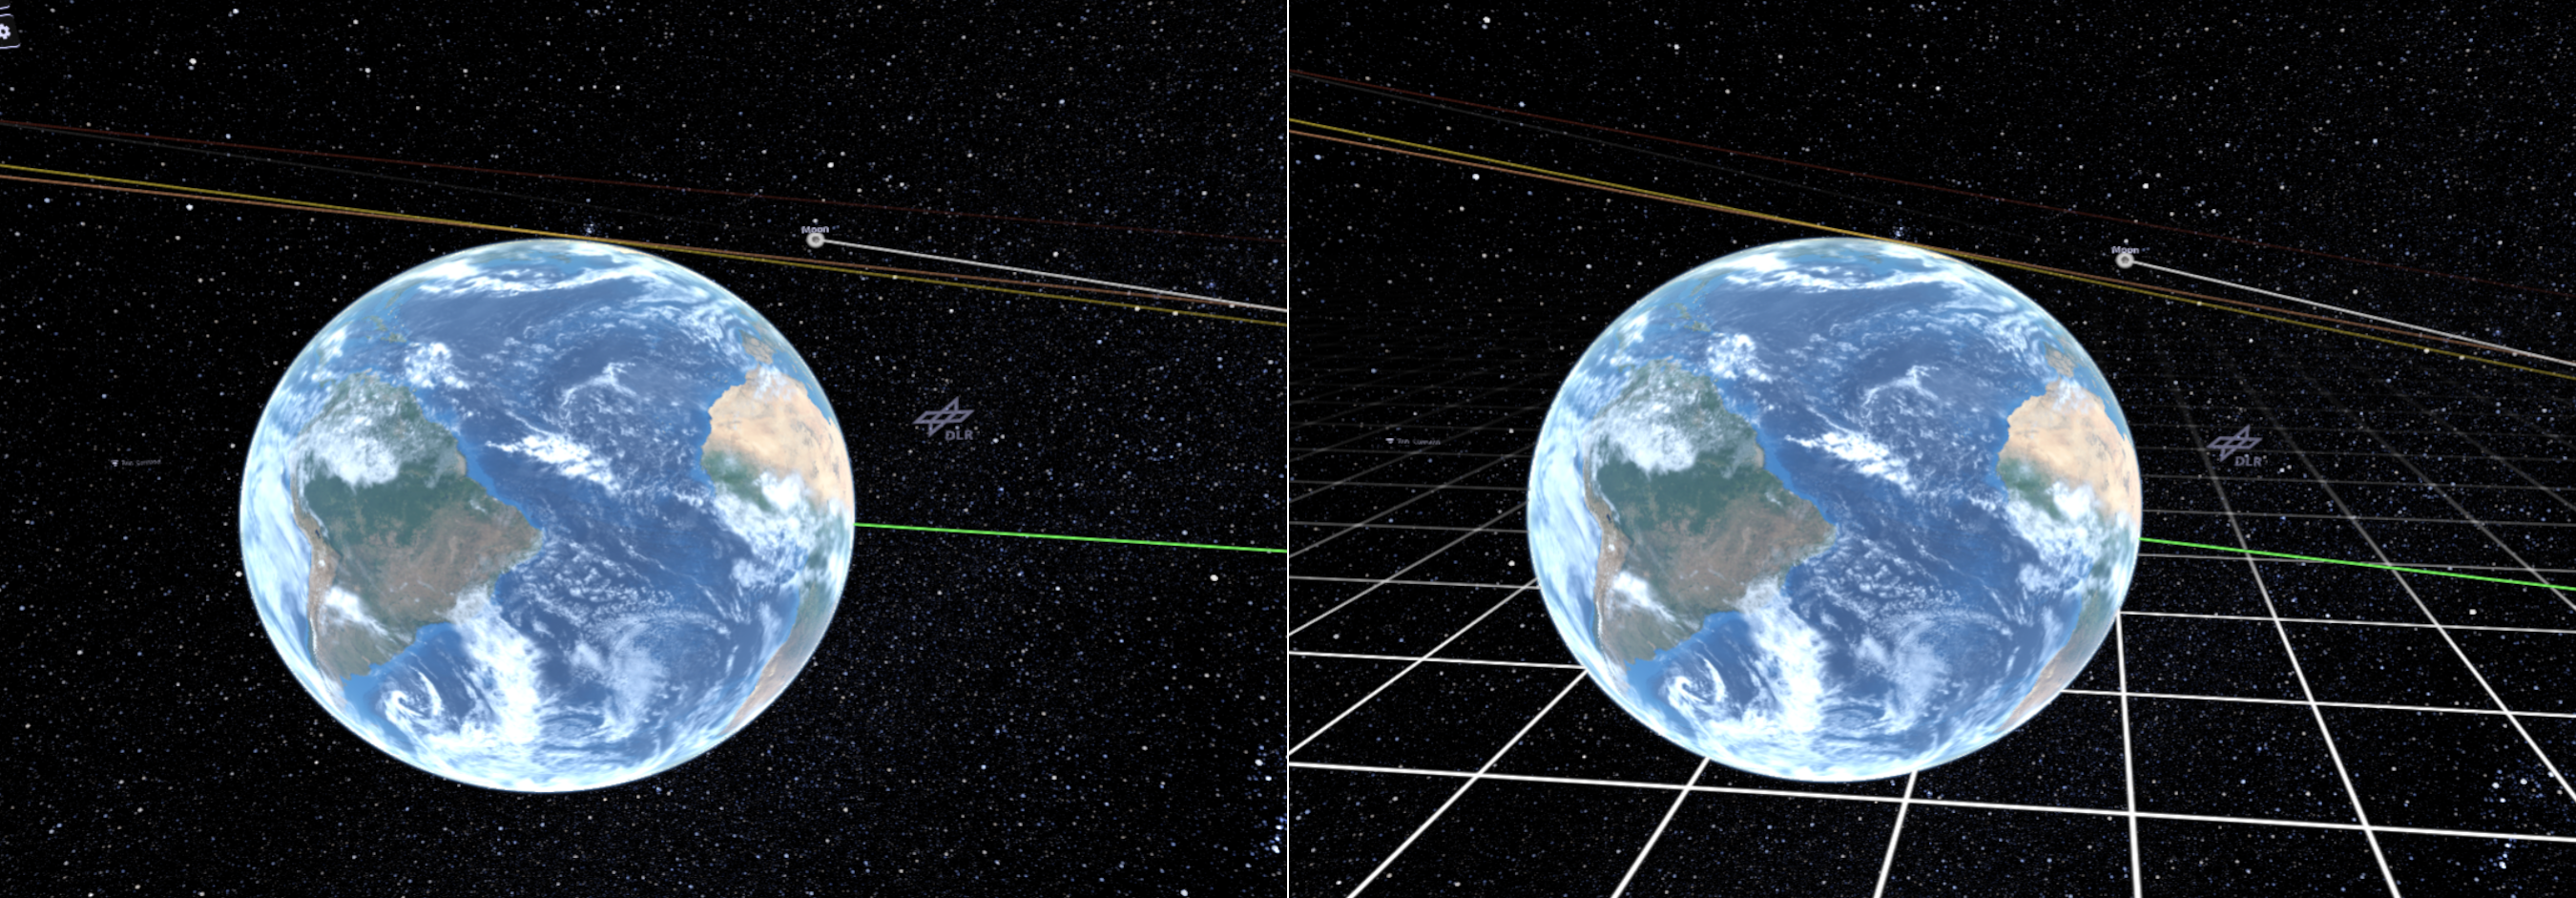
\includegraphics[width=\textwidth]{content/4_1_floorGrid/img/FloorGrid_Screenshot}
    \caption{Screenshot of CosmoScout VR without (left) and with (right) the Floor Grid.}
    \label{fig:floor-grid-screenshot}
\end{figure}

The Floor Grid is implemented in the VR Accessibility Plugin for CosmoScout VR, so it can be optionally loaded with
CosmoScout when it is needed and can be excluded in hardware setup where they are not.

It renders a quad that is fixed to the observer's position and GUI elements.
This way still allows free movements with the VR HMD while staying a static frame of reference that is tied to
the real world floor.
To properly adjust the grid to the real world floor the node drawing the quad is attached to the node drawing the GUI
via a transform node in the scenegraph that adds a vertical offset (in meters) to the grid that is adjustable in the
settings file before startup, and the options menu at runtime.

The quad size is defined in the settings file as a multiplier (\mintinline{c}{uFalloff}) that scales
the initial quad, spanning in x and y direction from -1 to 1, up by the value set in the settings file.
The scaled quad is textured with a semi transparent texture containing the grid with the center of the grid either as a
square or a cross.
Additionally, the texture can be scaled by a separate factor (\mintinline{c}{uSize}) resulting in a
coarser or finer mesh.

The calculations for the vertex positions and texture coordinates are shown in the code block below from the Floor
Grid's vertex shader:
\begin{minted}{c}
    void main() {
        vTexCoords  = vec2( (iQuadPos.x + 1)/2 * uFalloff * uSize,
                            (iQuadPos.y + 1)/2 * uFalloff * uSize );

        vPosition   = (uMatModelView * vec4(iQuadPos.x * uFalloff, 0.0, iQuadPos.y * uFalloff, 1.0)).xyz;
        gl_Position = uMatProjection * vec4(vPosition, 1);
    }
\end{minted}
The variables \mintinline{c}{uMatModelView} and \mintinline{c}{uMatProjection} are the Model, View, and Projection
Matrices needed to transform the coordinates in the graphics pipeline.

The Floor Grid's fragment shader applies the selected texture, but is discarded if the fragment is not part of a grid
line (i.e.\ is fully transparent).
Additionally, the texture's opacity (\mintinline{c}{uAlpha}) is adjustable through the settings file and
in the options menu at runtime.

To prevent aliasing or the grid turning into a grey plane towards the horizon, the floor grid is drawn with the
OpenGL Blend Function "\mintinline{c}{glBlendFunc(GL_SCR_ALPHA, GL_ONE_MINUS_SRC_ALPHA)}".
This blend function leads to the grid fading after a few meters because the texture is mostly transparent.
Finally, the color of the grid is adjustable in the settings file or in the options at runtime to allow more
customisation for individual users.

Figure~\ref{fig:floor-grid-screenshot} shows a screenshot of the floor grid in use compared to the same scene without
the grid.


\section{Field of View Vignette}\label{sec:field-of-view-vignette}

One of the most common methods to reduce cybersickness risks and symptoms is decreasing the Field of
View as examined in section~\ref{subsubsec:field-of-view-limitation}.
To alleviate cybersickness during movements with high detail, and movements in the peripheral areas of vision, a
vignette is implemented to limit the Field of View, focusing the users attention and preventing the influence of
activity in the peripheral vision from adding to cybersickness symptoms.


\subsection{FoV Vignette Concept}\label{subsec:fov-vignette-concept}

The Vignette is primarily planned for movements close to an object's surface, where peripheral visual flow is
significantly higher compared to movements in interplanetary space.

Additionally, reducing the FoV may help users during the adaption phase, by directing their view to the center of the
HMD's lenses where the image is focused.
While a point of interest is within a users field of view, they tend to shift their gaze without moving their head.
This can lead to users trying to focus on objects that are not at the center of their view, and thereby not in the
center of the HMD lenses.
In this case the user is trying to focus on part of the virtual environment, that cannot be focused on based on
hardware limitations.
A FoV vignette can help the adaptation process by limiting the FoV and nudging the user towards using head movements
instead of eye movements to look at different points of interest and keep their gaze centered at the middle of the
HMD's lenses.

Drogemuller et al.~\cite{Drogemuller2020} also recommend dynamically changing the FoV while using a one-handed
control scheme to reduce a users feeling of presence during complex movements in order to reduce discomfort.
However, these adaptation aids require a narrow FoV and may be perceived as limiting or annoying to other users.

According to the best practices by McCauley and Sharkey~\cite{McCauley1992}, and similar to the Floor Grid, the
vignette is designed to be modular and adaptable to each individual user.
Additionally, several options of vignetting are implemented, as suggested by Lim et al.~\cite{Lim2020}, to allow the
user options for both dynamic and fixed limitation of FoV\@.


\subsection{FoV Vignette Implementation}\label{subsec:fov-vignette-implementation}

\begin{figure}[h]
    \centering
    \includegraphics[width=\textwidth]{content/4_2_fovVignette/img/Vignette_Screenshot}
    \caption{Screenshot of CosmoScout VR without (left) and with (right) the FoV Vignette.}
    \label{fig:fov-vignette-screenshot}
\end{figure}

The FoV Vignette is also implemented in the VR Accessibility Plugin for CosmoScout VR, together with the Floor Grid.

The vignette is realized as a post-processing shader, drawing a 2D effect over the rendered scene based on an
inner and outer radius, which are both adjustable in the settings.
The inner radius determines the maximum distance from the center of the viewport, where a clear field of view is
guaranteed.
The outer radius determines the minimum distance from the center, above which the screen is fully opaque with a custom
color that is also adjustable in the settings.
The area between the inner and outer radius is bridged by a gradient, blending between fully transparent, showing the
rendered scene, and the fully opaque custom color at the outer radius.

Since the vignette is designed to block peripheral visual flow inducing vection and distracting the user during
movement, the vignette is only drawn during movement, and disabled when standing still or during sporadic, short
movements.
This allows reducing the risk of cybersickness symptoms during critical phases, while still maintaining the feeling
of presence as much as possible.
As mentioned above, two different methods of vignetting are implemented to offer more customization to the user, a
dynamic and a static vignette.

One method is drawing the vignette dynamically based on the observer's velocity in relation to the Observer's
position and distance to other bodies, as interplanetary movements allow for, and use significantly higher
velocities than movements close to a bodies surface.

For more customisation, an adjustable upper and lower velocity threshold for this normalized velocity is given to
allow more sensitive users an earlier and more noticeable vignetting, and more robust users the freedom to reduce its
effects.
The lower velocity threshold is the velocity at which the vignette will start limiting the FoV by decreasing its
radius, and the upper velocity threshold is the velocity where the vignette is at a determined minimum radius.
An adjustable threshold for the minimum velocity is used, since slow movements tend to only produce low risks of
cybersickness symptoms and limiting the FoV is usually not necessary.
Providing an upper velocity threshold serves solves two problems, it allows sensitive users to benefit of a
drastically reduced FoV as early as they feel comfortable, and additionally preventing the vignette from jittering
at maximum velocity where the velocity tends to fluctuate slightly, propagating to the radii of the dynamic vignette.

The FoV vignette is drawn in the same way for both options as shown in the fragment shader for the dynamic radius:
\begin{minted}{c}
    void main() {
        vec2 texSize = textureSize(uTexture, 0);
        float ratio  = texSize.y / texSize.x;

        float dist   = sqrt(vPosition.x * vPosition.x + ratio * ratio * vPosition.y * vPosition.y);

        if (dist < uInnerRadius ) { discard; }

        float r      = (dist - uInnerRadius) / (uOuterRadius - uInnerRadius);
        oColor       = mix(texture(uTexture, vTexCoords), uCustomColor, r);
        if (dist > uOuterRadius) {
          oColor.rgb = uCustomColor.rgb;
        }
    }
\end{minted}

First the distance (\mintinline{c}{dist}) of the current fragment to the center of the viewport is calculated and
adjusted for the viewport's aspect ratio (\mintinline{c}{ratio}).
Based on this distance and the inner and outer radius (\mintinline{c}{uInnerRadius} and \mintinline{c}{uOuterRadius})
the blending factor (\mintinline{c}{r}) is calculated, and the rendered scene (\mintinline{c}{uTexture}) is blended
with the custom color to create the gradient between the inner and outer radius.
If the fragment is inside the inner radius, the post processing is discarded,a nd if the fragment is outside the
outer radius it is set to the color of the vignette (\mintinline{c}{uCustomColor}).

The dynamic vignette's radius is controlled through the inner and outer radius that is passed to the fragment shader,
and is updated during the update frames of the simulation.
In the update the velocity is normalized to the upper and lower velocity threshold, and a new radius is calculated
partly based on the previous radius to dampen the propagation of harsh changes in velocity and smoothen the changes
in radii.
Currently, new radii propagate with a 1\% influence over each frame:
\begin{equation}
    \label{eq:radii-influence}
    r_{\mathrm{new}} = ( 0.99 \times r_{\mathrm{last}} ) + ( 0.01 \times r_{\mathrm{target}} )
\end{equation}

As suggested by Lim et al.~\cite{Lim2020}, a second option with a static vignette is also implemented.

The static vignette also uses the lower velocity threshold to determine when it should be drawn.
Additionally, an adjustable deadzone is implemented, allowing for a grace period where the vignette is not displayed
when passing the threshold to avoid flickering on short, quick movements, or velocities close to the threshold, that
pass the threshold when fluctuating slightly.
After passing the velocity threshold for at least the time specified in the deadzone or longer, a fade animation is used
to ease the vignette in or out over an adjustable duration, to make the transition to the limited field of view more
comfortable and less noticeable.

Through the use of an animation to gradually increase the opacity of the Vignette, a closing movement similar to the
dynamic vignette along the gradient is suggested.
However, the vignette is independent of the velocity, and is drawn with its specified minimum radius as soon as the
lower velocity threshold is passed.

As with the Floor Grid, almost all settings specifying the FoV vignette are adjustable either in the settings
file, or in the options menu at runtime, to allow users to customise the vignette according to their hardware setup
and preferences.

Finally, an experimental option is implemented, to only limit the FoV vertically and asymmetrically.

\begin{figure}[h]
    \centering
    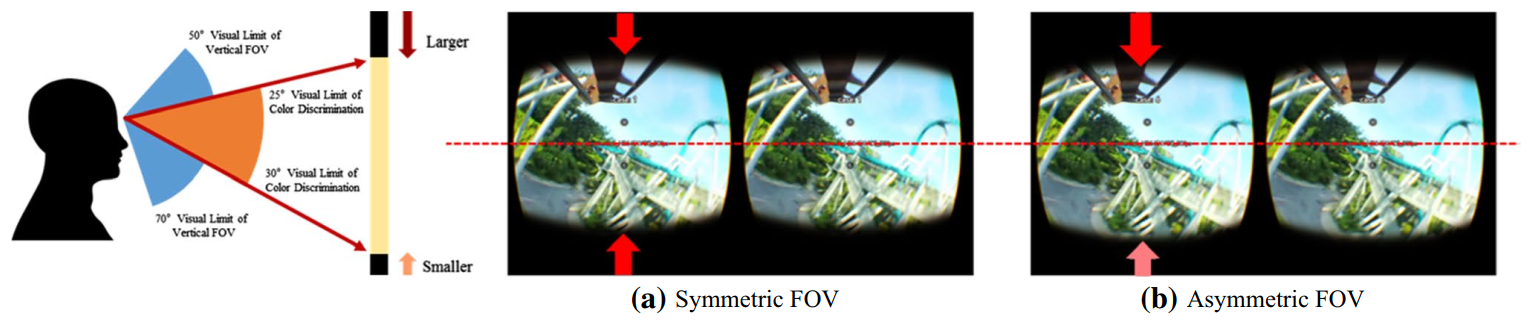
\includegraphics[width=\textwidth]{content/4_2_fovVignette/img/Asymmetrical_Vignette[Lim2020]}
    \caption{Asymmetrical FoV Limitation as proposed by Lim et al.~\cite{Lim2020}.}
    \label{fig:fov-assymetrical-vignette}
\end{figure}

Lim et al.~\cite{Lim2020} proposed in their study that the FoV vignetting should be applied asymmetrically, as human
visual characteristics produce an asymmetrical field of view with visual limits of 50\textdegree upwards and
70\textdegree downwards~\cite{Hatada1980}.
Since the horizontal field of view is significantly wider than the vertical field, we added an option to asymmetrically
limit the vertical field of view and forego any limitation of the horizontal visual field.

The fragment shader for the vertical vignette functions the same as their respective versions for the round
vignettes.
However, the calculation of the distance from the fragment to the center ignores the horizontal x-component as depicted
below:
\begin{minted}{c}
    float dist = 0;
    if (vPosition.y > 0) {
        dist = vPosition.y;
    } else {
        dist = vPosition.y * -0.7;
    }
\end{minted}
Instead of calculating the euclidean distance, the distance above the center is the vertical position of the fragment
from the center.
The distance below the center is multiplied by $0.7$ to result in a smaller distance, and thus a smaller vignette on
the bottom, as depicted in figure~\ref{fig:fov-assymetrical-vignette}.

This feature is implemented experimentally, mainly because Lim et al.\ implemented an asymmetrical FoV Limitation in
their study, but no symmetrical limitation.

We understand that Lim et al.\ as well as their reference Hatada, Sakata, and Kusaka~\cite{Hatada1980} argue for an
asymmetrical FoV vignette as it is based on human visual characteristics, and is therefore less noticeable.
However, an asymmetrical vignette could lead to users not focusing on the center of the HMD's lenses, but slightly
below, leading to unfocused images that may increase cybersickness symptoms.


\section{Automatic Movement Overhaul}\label{sec:automatic-movement-overhaul}

As pointed out in section~\ref{subsec:problems-with-automatic-movement}, the current automatic movement method was
built as temporary means to navigate between saved bookmarks.
The method applies a linear interpolation to transition smoothly between the origin and target position leading to
movement in a straight line between the two points.
Additionally, a linear interpolation between the origin and target orientation is used to rotate the observer into the
target orientation.
While this is the easiest, and most straightforward way to smoothly move the observer through the simulation without
breaking continuity by teleporting the user, the simultaneous translation and rotation have been found to induce
disorientation followed up by motion sickness symptoms by the user.

In this section a new automatic navigation for CosmoScout is presented, which aims to make the automatic navigation
more accessible and less sickness inducing.
As parts of the navigation have not been fully implemented, we first present the concepts how the automatic
navigation system should move the observer.
After the concept, key features of the implemented solutions are presented and explained.


\subsection{Automatic Movement Concept}\label{subsec:automatic-movement-concept}

The main goal, found to reduce cybersickness for automatic movement, is reducing the complexity of the movement by
decoupling the rotation from the translation.
This way the movements are easier to read, and the user should be able to better anticipate the observers movements,
reducing motion sickness symptoms.

First, the linear interpolation is exchanged for movement along a spline.
This way, it does not change the linear movement between points in space as it was implemented before, while still
accomodating for different, non-linear paths the observer can take.
Additionally, this change is made to facilitate more variability for later development, like programmed virtual tours
along points of interest.
Additionally, the change to splines is made to enable easier collision handling for the navigation method, as
additional control points can be inserted to handle collisions and divert the movement path.

Since the origin and target location and orientation of the automatic navigation can be arbitrary points anywhere in
the simulation (both bookmarked and calculated intermediate locations), the first step is to classify the possible
locations into groups.
We propose the classification of locations based on their location relative to other bodies, and the SPICE reference
frame the location is in:
\begin{itemize}
    \item Surface locations, that are extremely low orbit, or on the surface of a body, where the location's position
    and orientation are in the respective body's SPICE frame relative to the body's center;
    \item Orbit locations, where the location is further from the surface, but the position and orientation
    are still relative to the body's SPICE center;
    \item Interplanetary locations, where the location's position and orientation is not relative to another body's
    SPICE frame and center, but the solar system's barycenter, i.e.\ the "J2000" SPICE frame.
\end{itemize}
Through the classification of locations a set of general movements and transitions can be derived to access all of
those locations in a manner that is predictable for the user, while still general enough to minimize special cases
that could lead to unwanted behaviour.

The classification of locations leads to 3 types of movement and the transitions between them, resulting in the states
shown in figure~\ref{fig:nav-states}.

\begin{figure}[h]
    \centering
    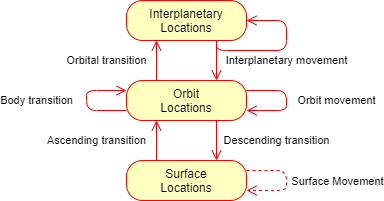
\includegraphics[width=0.5\textwidth]{content/4_3_autoNavigation/img/NavigationLocationStates}
    \caption{State diagram for the different types of locations, and the movements and transitions between them.}
    \label{fig:nav-states}
\end{figure}

The different movements are structured in layers, therefore a transition from surface to interplanetary space and
vice versa is done via transition from surface to orbit, and from orbit to interplanetary space.
Additionally, there is no explicit transition from interplanetary movement to orbital movement since the interplanetary
movements end in a position where either the destination is reached, or the observer is in a position in the target
orbit and is able to resume orbital movement immediately.

An example for this layered travel is a movement from a location on the origin body's surface to a location on the
target body's surface:
the movement starts in the "Surface movement" state, since the origin location is on a body's surface.
First, the observer transitions from the surface location to an orbit location via the ascension transition, because
the observer is still in the origin's SPICE frame.
Then, since the observer is still in the wrong frame, the observer transitions to a position for interplanetary
movement, and moves to towards the target via interplanetary movement, ending in an orbital location in the target
frame.
Then, an orbital movement is performed to move above the final location on the surface.
Finally, the observer enters a decension transitions to the final location on the surface.

While a SPICE frame is merely a nested oriented frame of reference, and therefore not limited in distance from its
center, in the context of the navigation concept, the frame is used as a general reference to a body's sphere of
influence, where the observer is eiter on the surface or in an arbitrarily, but reasonably high orbit around the body.

\subsubsection{Surface Movement}\label{subsubsec:surface-movements}

\begin{wrapfigure}{o}{0.25\textwidth}
    \centering
    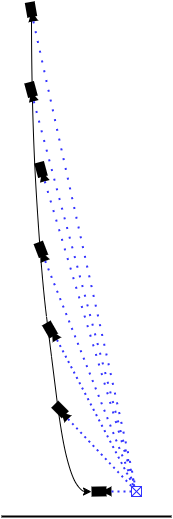
\includegraphics[width=0.1\textwidth]{content/4_3_autoNavigation/img/PlannedLanding}
    \caption{Planned automatic movement descending onto a body's surface.}
    \label{fig:new-auto-nav-descend}
\end{wrapfigure}

In this overhaul, we did not primarily focus on a solution for automatic movement on the surface of a body, since
those movements are strongly dependent on distance and topology between the target and origin.
Additionally, surface navigation is difficult to test under the current circumstances, since a connection to the DLR
map server is needed to poll street level elevation data and textures, and both were unavailable in the remote work
setting due to the COVID-19 pandemic.
In order to find a general solution, independent of distance and topology, we chose to facilitate surface movements
via orbital travel, i.e.\ transitioning from the surface origin location into orbit, using orbital movement to go to an
orbital location above the target surface location and transitioning back down to the surface at the target location.
While this solution may be inconvenient for short distances relative to the body's circumference, we assume this form
of movement to be a default solution independent of topology or distance.
Further solutions for surface movements, especially for short distances, should be easily implementable in later
works using the established framework we develop here.

The important changes in the surface movement are the transitions between surface and orbit (the landing and
ascending movements).
In order to prevent the change of reference frame, as pointed out in
section~\ref{subsec:problems-with-automatic-movement}, we plan to change the linear path and simultaneous rotation
shown in figure~\ref{fig:old-auto-nav-descend}, to a parabolic curve, so the observer's movements are always
perceived as forward, not downward, and the observer swoops into the target location on the surface, as depicted in
figure~\ref{fig:new-auto-nav-descend}.
To ease the rotation and enable the user to predict the movement, the center of the viewport is aimed at a point
slightly in front of the final position in direction of the final orientation.
This essentially separates the translation from the rotation due to the steepness of the movement.
The bulk of the rotation during the movement is at the end of the curve where the curvature is highest.

The ascending transition is basically similar, but in reverse, so the observer zooms out moving backwards and
focusing on the point of origin until it reaches the default orbital distance where the point of origin should almost
coincide with the body's center.

\subsubsection{Orbital Movement}\label{subsubsec:orbital-movements}

The default orbital distance for each body is relative to the body size, so that the orbited body always occupies the
same space of the viewport, independent of the body's size.
In order to prevent movements through the body as shown in figure~\ref{fig:old-auto-nav-collision} in
section~\ref{subsec:problems-with-automatic-movement}, we plan to use the flexibility of splines to move the observer
in circular curves around the body, while focusing the center of the viewport on the center of the body.

While this movement has simultaneous translation and rotation, this movement is not perceived by most users as the
observer moving around the body, but a rotation of the whole simulation around the body where the viewport is focused
on.
In case either the starting point, or the final location are not equidistant to the boday's center, the curve becomes
less circular, but the nature of the spline should compensate for different distances to the center automatically,
leading to the user perceiving the change in distance as the observer zooming out, away from the body during the
rotation.

For the transition from orbital to interplanetary movement, a few steps are added to reduce surprising rotations and
make the movement easier to predict by the user.

\begin{figure}[h]
    \centering
    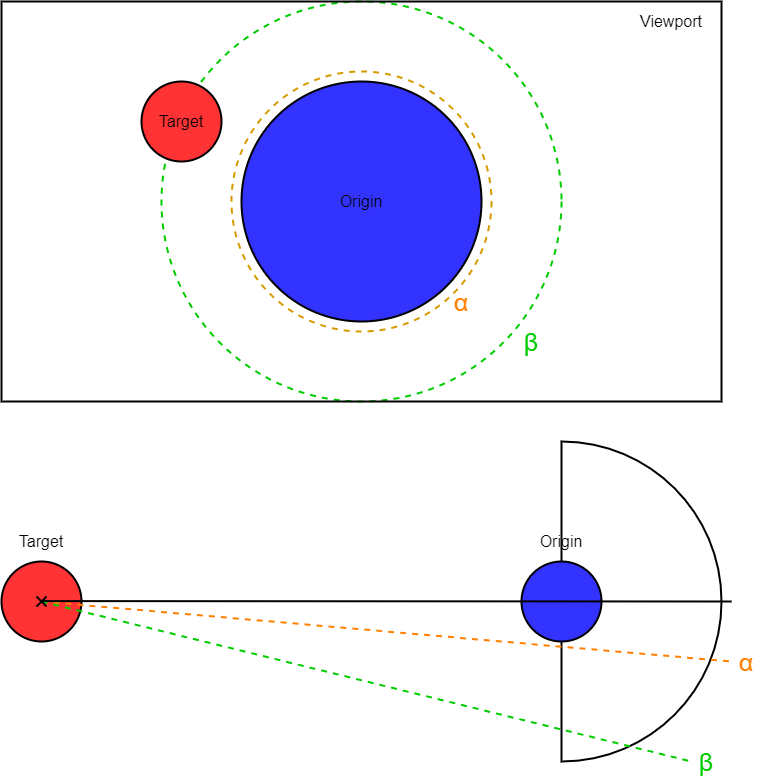
\includegraphics[width=0.66\textwidth]{content/4_3_autoNavigation/img/OrbitTransitionAngles}
    \caption{Minimum ($\alpha$) and maximum ($\beta$) angle for the transition into interplanetary movement.}
    \label{fig:orbital-transition-angles}
\end{figure}

First, the observer finds the closest suitable location where the following conditions are met:
\begin{itemize}
    \item The angle $\theta$ between the vector from the target's center to the observer, and the vector from the
    target's center to the origin's center is between the minimum allowed angle $\alpha$ and the maximum allowed
    angle $\beta$.
    \begin{equation}
        \label{eq:orbital-angles}
        \alpha \geq \theta \geq \beta
    \end{equation}

    \item The vector $\vec{v}$ between the target's center, and the observer must be longer than the vector $\vec{w}$
    between the target's center, and the origin's center.
    \begin{equation}
        \label{eq:orbital-magnitudes}
        \left\| \vec{v} \right\| > \left\| \vec{w} \right\|
    \end{equation}
\end{itemize}
The requirements are visualised in figure~\ref{fig:orbital-transition-angles}.
The first requirement (equation~\ref{eq:orbital-angles}), creates two cones from the target's center towards the origin.
The $\alpha$-cone is the minimum angle, that prevents the target from being mostly obscured by the origin body, and
the $\beta$-cone is the maximum angle, that ensures the Target is still visible on the viewport.
Both cones intersect the sphere of the origin's possible orbit locations twice, resulting in two spherical segments.
The second requirement excludes the spherical segment that is in between the origin and target bodies.
The spherical zone of the remaining segment are the available locations for the interplanetary transitions,
figure~\ref{fig:orbital-transition-zone} visualises the possible locations.

\begin{wrapfigure}{o}{0.25\textwidth}
    \centering
    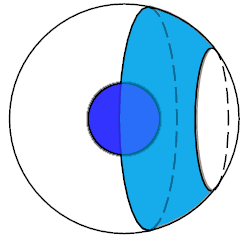
\includegraphics[width=0.2\textwidth]{content/4_3_autoNavigation/img/OrbitTransitionSphericalZone}
    \caption{Spherical zone of locations available for the interplanetary transition.}
    \label{fig:orbital-transition-zone}
\end{wrapfigure}

The transition for interplanetary movement is to move to the closest location in this spherical zone via orbital
movement, which results in a scene similar to the viewport in figure~\ref{fig:orbital-transition-angles}, where the
viewport is focused on the center of the origin's body, and the target body is within the $\alpha$ and $\beta$
margins in the viewport.

\subsubsection{Interplanetary Movement}\label{subsubsec:interplanetary-movement}

The interplanetary movement remains closest to the original movement.
However, the interpolation between the origin and target orientation is removed in order to separate rotation from
translation and increase predictability.
Instead, the rotation is split into an initial rotation to fave the traveling direction, so the user always moves
forward, towards the target, and a final rotation at the end of the translation to rotate the observer into the final
orientation at the target location.

The translation uses a straight spline.
This way the movement is similar to the original interpolation between the origin and target position.
However, the spline allows easier modification of the path, leading to easier collision detection and mitigation in
the future, since the spline can be easily checked for collisions and, if necessary, additional control points can be
inserted into the spline to avoid collisions.
The interplanetary movement always ends in either an interplanetary location (bookmark) or a target body's orbit,
where orbital movement can be resumed.
Therefore, no transition from interplanetary movement to orbital movement is needed.

\begin{figure}[h]
    \centering
    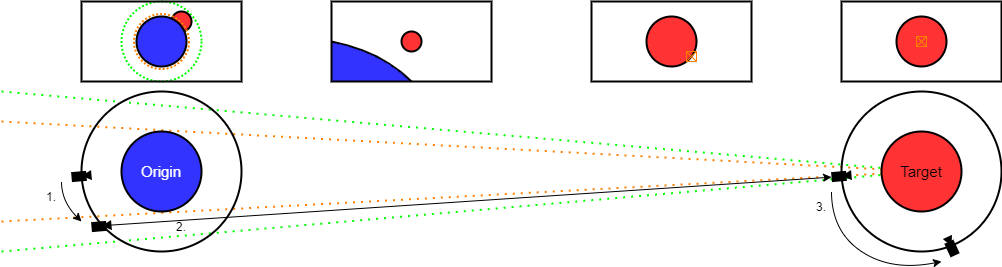
\includegraphics[width=\textwidth]{content/4_3_autoNavigation/img/Orbit2OrbitExample}
    \caption{Example of automatic movement including the orbital to interplanetary movement transition (1.), the
    interplanetary movement (2.), and orbital movement the the final position (3.).}
    \label{fig:orbital-example}
\end{figure}

An example of movement between two orbital locations, is shown in figure~\ref{fig:orbital-example}.
The first step shown in the figure is the transition from an arbitrary orbital location around the origin body to a
location that fulfills the requirements (equations~\ref{eq:orbital-angles}~\&~\ref{eq:orbital-magnitudes}).

The second step is the interplanetary movement between the origin orbit, and the target orbit.
First, the observer rotates from focusing on the origin's center to the target's center, and travel direction.
During this rotation the requirements for the transition between orbital and interplanetary movement, help reduce the
angular distance of the rotation and prevent collision with the origin body during interplanetary travel.

After arriving at the target's orbit, the third step is an orbital movement to the final position.

While this staged approach increases the overall travel time of the automatic navigation, we aim to reduce
disorientation and resulting cybersickness symptoms by providing the user with an easily predictable solution that
decouples rotation from translation and minimizes complex and surprising rotations.


\subsection{Automatic Movement Implementation}\label{subsec:automatic-movement-implementation}

The automatic movement for CosmoScout is organized in two distinct parts.
The first part is the \mintinline{c}{moveTo}-method, where the parameters of the movement are processed, and the second
part is the \mintinline{c}{updateMovementAnimation}-method which is called every frame, polling the state of the
movement based on the current time.

The old \mintinline{c}{moveTo}-method uses the information about the current position and orientation for the origin, as
well as the parameter information about the target location, and the duration of the movement to construct two
\mintinline{c}{AnimatedValue} objects.

An \mintinline{c}{AnimatedValue} object is consists of a start and end value, as well as a start and end time.
The object then provides a method to poll the value using time as the parameter, returning either the start or
end value, if the time is outside the timespan provided by the start and end time of the
\mintinline{c}{AnimatedValue}, or the method returns an interpolated value between the start and end values relative
to the point in time between the start and end time.

One \mintinline{c}{AnimatedValue} is used for the translation, interpolating between the origin
position, and the target position over the duration of the movement.
The other \mintinline{c}{AnimatedValue} is used for the rotation, interpolating between the origin orientation and the
target orientation over the duration of the movement.

After the \mintinline{c}{moveTo}-method has processed the available information into the two
\mintinline{c}{AnimatedValue} objects, the \mintinline{c}{mAnimationInProgress} flag is set.
While the flag is true, the \mintinline{c}{updateMovementAnimation}-method uses the current time at each frame to
poll the current position and orientation from the \mintinline{c}{AnimatedValue} objects, until the time is past the
end time of both end times.
Afterwards, the \mintinline{c}{updateMovementAnimation} resets the \mintinline{c}{mAnimationInProgress} flag to false.

Since the automatic movement can potentially be called from anywhere in CosmoScout, including plugins, we plan to
ensure backwards compatibility while changing the way the automatic movement is performed.
Therefore, the original \mintinline{c}{moveTo}-method's signature is kept and additional signatures are added as needed.
The original \mintinline{c}{moveTo}-method was an interpolation between the origin and target location leading to a
linear movement path from the origin to the target.
Since the interplanetary movement shows similar characteristics, the \mintinline{c}{moveTo}-method that contains the old
method signature is also used for interplanetary travel, and generally linear movements.

The first change to the method is replacing the \mintinline{c}{AnimatedValue} object for the interpolation of the
observers position with a linear spline between the origin and target position, and using the
\mintinline{c}{AnimatedValue} object to interpolate the $t$ parameter over the length of the spline relative to the
duration of the movement.

Second, split the rotation into an initial rotation, from the origin orientation to a \mintinline{c}{mLookAtPoint} in
movement direction, and a final rotation, from the \mintinline{c}{mLookAtPoint} to the final orientation.
Additionally, the rotations are separated from the translation by adjusting the start and end times of the
\mintinline{c}{AnimatedValue}-objects.

The overall duration ($t_{all}$) is split into three stages, the initial rotation ($t_{start}$), the translative phase
($t_{move}$), and the final rotation ($t_{end}$).
For the duration of each rotation a function (equation~\ref{eq:duration-weight}) is used that calculates a weight
factor ($w$) between 0 and 1 based on the angular difference ($\theta$) of the start and the end direction of view
(negative $z$-axis).
This way, the durations for each rotation can vary in length based on the angular difference of the rotation, and the
translative phase takes up the rest of the duration as described in the following equations:
\begin{equation}
    \label{eq:duration-timings}
    \frac{w_{\mathrm{start}}}{3} t_{\mathrm{start}} + (1 - \frac{w_{\mathrm{start}}}{3} - \frac{w_{\mathrm{end}}}{3})
    t_{\mathrm{move}} +
    \frac{w_{\mathrm{end}}}{3} t_{\mathrm{end}} = t_{\mathrm{all}}
\end{equation}
with:
\begin{equation}
    \label{eq:duration-weight}
    w = f(\theta) = - \frac{\cos{\theta} - 1}{2}
\end{equation}
This results in the following limitations for the durations:
\begin{equation}
    \label{eq:duration-result-rot}
    0 \leq t_{\mathrm{start}}, t_{\mathrm{end}} \leq \tfrac{1}{3} t_{\mathrm{all}}
\end{equation}
\begin{equation}
    \label{eq:duration-result-mov}
    \tfrac{1}{3} t_{\mathrm{all}} \leq t_{\mathrm{move}} \leq t_{\mathrm{all}}
\end{equation}

The modifications to the \mintinline{c}{moveTo}-method also require changes to the
\mintinline{c}{updateMovementAnimation}-method, as the position and rotation needs to be polled from different sources.
Additionally, the simulation is changed to stop the simulation time during movement.
The automatic movement is programmed to transform all positions into the target's SPICE frame, and the delay of the
initial rotation before translation results in inadvertent movement, as the target frame rotates, moving the observer
significantly due to the distance to the target's center.

\subsubsection{Changes to \mintinline{c}{updateMovementAnimation}}\label{subsubsec:changes-to-updatemovementanimation}

\begin{minted}{c}
    void CelestialObserver::updateMovementAnimation(double tTime) {
        if (mAnimationInProgress) {
            // get position from spline
            mPosition = mMoveSpline->getPosition(mAnimatedT.get(tTime));

            if (tTime < mAnimatedRotationStart.mEndTime) {
                // rotation to look-at point not done yet
                mRotation = mAnimatedRotationStart.get(tTime);
            } else if (tTime > mAnimatedRotationFinal.mStartTime) {
                // rotation to final direction started
                mRotation = mAnimatedRotationFinal.get(tTime);
            } else {
                // observer is moving along spline -> adjust rotation towards look-at point
                auto direction = glm::normalize(mLookAtPoint - mPosition);
                mRotation      = glm::quatLookAt(direction, mUpDirection);
            }

            if (mAnimatedRotationFinal.mEndTime < tTime) {
                mAnimationInProgress = false;
                if (!mMovementQueue.empty()) {
                    moveTo(mMovementQueue.front());
                    mMovementQueue.pop();
                }
            }
        }
    }
\end{minted}
The polling of the current position only has minimal changes (l.\@4), as the \mintinline{c}{AnimatedValue}
is polled to receive the $t$ parameter for the position on the spline based on the current time, instead of receiving
the interpolated position directly from the \mintinline{c}{AnimatedValue}.

Polling the orientation is dependent on the current time in the movement process (ll.\@6--16).
If the current time is before the end time of the initial rotation, the current orientation is provided by the
\mintinline{c}{AnimatedValue} of the initial rotation, interpolating between the original orientation, and the
orientation towards the \mintinline{c}{mLookAtPoint}.
If the current time is after the start time of the final rotation, the orientation is provided by the
\mintinline{c}{AnimatedValue} of the final rotation, interpolating between the orientation aimed at the
\mintinline{c}{mLookAtPoint}, and the final orientation.
Otherwise, the movement animation is in the translative phase, and the current orientation is calculated using the 
\mintinline{c}{mLookAtPoint}, and the \mintinline{c}{mUpDirection} to generate a new orientation focused on the
\mintinline{c}{mLookAtPoint}.
The \mintinline{c}{mUpDirection} is saved from the orientation of the observer at the beginning of the movement
animation, to prevent the camera from any rolling rotations during the movement animation, since rolling during
movements appears to increase disorientation and therefore discomfort in users.
Lines 18--24 of the code block contain another important change that is explained in the next section.

\subsubsection{Movement Description Packages and Movement Queue}\label{subsubsec:movement-description-packages-and-movement-queue}

Based on the new changes to the \mintinline{c}{updateMovementAnimation}-method, there are the following requirements any
movement must fill with data in order for the movement animation to display correctly:
\begin{itemize}
    \item The \mintinline{c}{mMoveSpline}, providing the path for the movement, and the \mintinline{c}{AnimatedValue}
    for the interpolation of the $t$ parameter for the spline.
    \item The \mintinline{c}{AnimatedValue} for the initial rotation from the origin direction towards the
    \mintinline{c}{mLookAtPoint}.
    \item The \mintinline{c}{mLookAtPoint} to focus on during the translation, and the \mintinline{c}{mUpDirection}
    to calculate the orientation and prevent rolling.
    \item The \mintinline{c}{AnimatedValue} for the final rotation from the direction towards the
    \mintinline{c}{mLookAtPoint} to the final direction.
\end{itemize}
Any new movement must provide these information and therefore, a movement always consist of the initial rotation,
then the translation with a given point focused in the center of the viewport during the movement, and a final
rotation into the final orientation.

To provide functionality for the transitions, as well as future, potentially complex movements and routes, a queue is
added to the automatic movement system.
The parameters needed by the \mintinline{c}{moveTo}-methods to process into the above mentioned requirements are
packaged into structs, and the \mintinline{c}{mMovementQueue} provides a FIFO queue to hold an ordered list of these
movement instructions.
At the end of the \mintinline{c}{updateMovementAnimation}-method (ll.\@18--24), the
\mintinline{c}{mMovementQueue} is checked whether it contains any items, and if so, the topmost item is removed, and the
\mintinline{c}{moveTo}-method is called with the struct as parameter.
For this additional \mintinline{c}{moveTo}-methods can be added to provide different types of movement.
Additionally, a \mintinline{c}{moveTo}-method is added that accepts a queue of movement instructions as a parameter, as
shown below:
\begin{minted}{c}
    void CelestialObserver::moveTo(std::queue<MovementDescription> const& moveDescriptionsQueue) {
        // make sure queue contains at least one element
        if (!moveDescriptionsQueue.empty()) {
            // swap new movements into queue
            mMovementQueue = moveDescriptionsQueue;
            // execute first movement instruction
            moveTo(mMovementQueue.front());
            mMovementQueue.pop();
        }
    }
\end{minted}
Providing a new, non-empty queue to the method during an ongoing movement discards remaining items, emplaces the
new queue into the \mintinline{c}{mMovementQueue}, and calls the \mintinline{c}{moveTo}-method with the topmost item
of the queue.
Discarding the old queue when receiving a new queue is done, to prevent buffering of multiple, potentially unwanted
movements.

\begin{figure}[h]
    \centering
    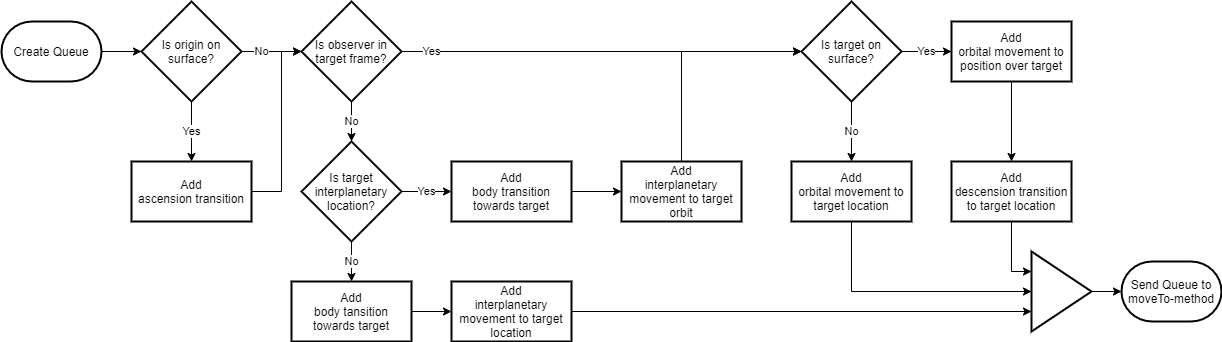
\includegraphics[width=\textwidth]{content/4_3_autoNavigation/img/QueueConstructionFlowchart}
    \caption{Flowchart for the construction of a movement queue.}
    \label{fig:movement-queue}
\end{figure}

Currently, the \mintinline{c}{mMovementQueue} can be filled with a variant of the two basic movement description
packages.
Either the linear movement that resulted from the original \mintinline{c}{moveTo}-method, and is used in the
interplanetary movement, or the circular movement that is used in the orbital movement.
The construction of a movement queue based on information about origin and target location is shown in the
flowchart in figure~\ref{fig:movement-queue}.

\subsubsection{Different \mintinline{c}{moveTo}-methods and Control Point Computation}\label{subsubsec:different-moveto-methods-and-control-point-computation}

To provide different types of movement, the \mintinline{c}{moveTo}-method has multiple implementation with different
signatures:
\begin{minted}{c}
    void moveTo(std::string const& centerName, std::string const& frameName,
        glm::dvec3 const& position, glm::dquat const& rotation, double simulationTime,
        double realStartTime, double realEndTime);

    void moveTo(DefaultPoint2Point const& moveDescriptionP2P);

    void moveTo(DefaultOrbit const& moveDescriptionOrbit);

    void moveTo(MovementDescription const& moveDescription);

    void moveTo(std::queue<MovementDescription> const& moveDescriptionsQueue);
\end{minted}
The original signature of the method (l.\@1) is kept to allow backwards compatibility.
The second signature (l.\@5) accepts movement description packages for linear, point-to-point (interplanetary)
movements.
The function simply unpacks and relays the parameters for the linear movement to the first \mintinline{c}{moveTo}-method.
The third signature (l.\@7) accepts movement description packages for circular (orbital) movements.
The fourth signature (l.\@9) is added because the movement queue uses a variant type for its elements.
Therefore, when a new element for the queue is used, this method accepts it.
The method checks the real movement description type using a switch-case-statement, and typecasts the variant-type
elements, and relays them to their respective methods.
The last signature (l.\@11) accepts whole movement queues to be passed and is described above.
Currently, only linear and circular movement packages are implemented, however, the addition of further movement
description packages is straightforward in this system.

The movement path is constructed using a uniform cubic basis splines.
Uniform cubic b-splines offer some advantages over other curves, as they are similar to bezier curves, which means
they are relatively easy to construct, and have a continuous velocity over the curve.
Additionally, uniform cubic b-splines offer a continuous curvature, easing the movement of the observer along the
spline.
Lastly, their control points only have local influence on the curve, which means that additional control points can
be inserted to handle collisions, without major changes to the overall curve.
Their only disadvantage, the interpolated curve not necessarily passing through the specified control points, can be
mitigated by inserting triplets of control points with the middle point being the control point teh curve should pass
close to, and the other two points representing a tangent to the curve that is passing through the three control points.

Uniform cubic b-splines that are non-looping also require an additional point on either end of the curve where the
curve is not interpolated.
Therefore, the curve for the movement always starts in the second and ends in the penultimate control point.

The spline for the interplanetary movement is constructed between the origin and target using two triplets of control
points.

\begin{figure}[h]
    \centering
    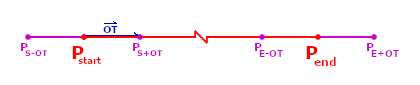
\includegraphics[width=0.5\textwidth]{content/4_3_autoNavigation/img/LinearSplinePoints}
    \caption{Control points of a linear spline with the start and end point ($P_{\mathrm{start}}$,
        $P_{\mathrm{end}}$), and the control points ($P_{S-OT}$, $P_{S+OT}$, $P_{E-OT}$, $P_{E+OT}$) making up each
        triplet.}
    \label{fig:linear-control-points}
\end{figure}

First, the vector between the origin and target ($OT$-vector) is constructed and normalized.
Then, each triplet forms the tangent through the start and end point, where the start or end point is the middle
control point, with one control point in front, and one control point behind the middle point in direction of the
$OT$-vector, as described in figure~\ref{fig:linear-control-points}.
This way, bot the tangent in the start and end point are along the $OT$-vector, leading to a straight spline between
the start and end point.
The resulting spline is saved in the \mintinline{c}{mMoveSpline}, and the \mintinline{c}{AnimatedValue}-object for the
interpolation of the $t$ parameter is set to interpolate between $0$ and $t_{\mathrm{max}}$ ($1$ in most cases) over the
duration of the translation phase.

The \mintinline{c}{mLookAtPoint} is set to the last control point, as it is slightly in front of the end point of the
interpolated spline.
This way the observer is always oriented towards the end point of the movement path, without the movement ending in a
location where the position and \mintinline{c}{mLookAtPoint} coincide, which could lead to an undefined orientation
for the observer.
Additionally, the \mintinline{c}{mUpDirection} is saved from the up-direction of the observer in the origin location to
prevent the observer from rolling during the movement phase.

Finally, the \mintinline{c}{AnimatedValue}-objects for the initial, and the final rotation are set.
The initial rotation interpolates between the origin orientation, and the orientation towards the
\mintinline{c}{mLookAtPoint} over the duration for the initial rotation.
The final rotation interpolates between the orientation towards the \mintinline{c}{mLookAtPoint} and the final
orientation over the duration for the final rotation.

The durations and points in time for the rotations, and the translation are calculated as mentioned above
(equations~\ref{eq:duration-weight}~and~\ref{eq:duration-timings}).

The orbital movement uses a different \mintinline{c}{moveTo}-method to realize the circular movement path.
To approximate the circular arc between the start and end point, both points are projected into 2D space by finding
the normal to the plane defined by the center-start, and center-end vectors ($\overrightarrow{cs}$ and
$\overrightarrow{ce}$).
This also results in the shortest possible path in orbit from the start to the end point.
Next, the angle ($\theta$) between the two vectors is calculated, and both vectors are normalized to compute the
additional control points on the unit circle.

\begin{figure}[h]
    \centering
    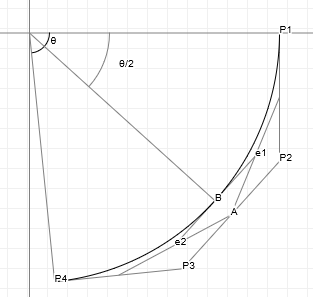
\includegraphics[width=0.5\textwidth]{content/4_3_autoNavigation/img/CircularCurveParameters}
    \caption{Control points ($P2$, $P3$), the start point ($P1$), end point ($P4$) and angle ($\theta$) in 2D
    space~\cite{Pomax2021}.}
    \label{fig:orbital-control-points}
\end{figure}

Figure~\ref{fig:orbital-control-points} shows an example of the transformation into 2D space, and the required
control points ($P1$, $P2$, $P3$, and $P4$).
Pomax~\cite{Pomax2021} derived a formula to calculate the missing control points $P2$ and $P3$ on the unit circle:
\begin{equation}
    \label{eq:control-points}
    \begin{aligned}
        P_{\mathrm{start}} &= P1 = (1, 0) \\
        P_{c1} &= P2 = (1, k) \\
        P_{c2} &= P3 = (\cos(\theta) + k \cdot \sin(\theta), \sin(\theta) - k \cdot \cos(\theta)) \\
        P_{\mathrm{end}} &= P4 = (\cos(\theta), \sin(\theta))
    \end{aligned}
\end{equation}
With:
\begin{equation}
    \label{eq:control-points-factor}
    \begin{aligned}
        k &= f(\theta) = \frac{4}{3} \cdot \tan\left( \frac{\theta}{4} \right)
    \end{aligned}
\end{equation}
To transform the control points back into 3D space, the oriented angle around the center from $P1$ to $P2$
($\phi_{\mathrm{start}}$), and from $P4$ to $P3$ ($\phi_{\mathrm{end}}$) is calculated.
To get the control points, the start position and end position are rotated around the normal of the 2D plane, and
scaled by the magnitude of their 2D counterpart.

\begin{figure}[h]
    \centering
    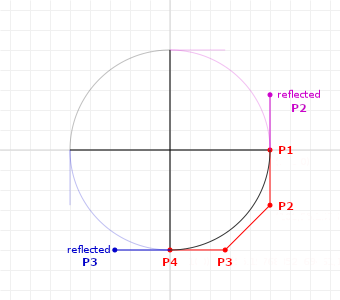
\includegraphics[width=0.5\textwidth]{content/4_3_autoNavigation/img/ControlPointsReflected}
    \caption{Example control points for circular spline where $\theta = 90\deg$~\cite{Pomax2021}.}
    \label{fig:orbital-reflected-points}
\end{figure}

Since, the spline needs two additional control points where the spline is not interpolated, the calculated control
points are also reflected to the other side of the start and end position as shown in
figure~\ref{fig:orbital-reflected-points}.

The control points in 3D space ($C_{P2}$, $C_{P3}$), and their reflections ($C_{rP2}$, $C_{rP3}$) can be calculated
using Rodrigues' rotation formula with the start and end points ($C_{\mathrm{start}}$, $C_{\mathrm{end}}$), the
normal for the 2D plane ($\vec{N}$), the angles between the control point, and the start, or end point
($\phi_{\mathrm{start}}$, $\phi_{\mathrm{end}}$), and the control points in 2D space ($\overrightarrow{P2}$,
$\overrightarrow{P3}$):
\begin{equation}
    \label{eq:control-point-transformation}
    \begin{aligned}
        \vec{C}_{P2} &= \left(
            \vec{C}_{\mathrm{start}} \cos(\phi_{\mathrm{start}}) +
            ( \vec{N} \times \vec{C}_{\mathrm{start}} )\sin(\phi_{\mathrm{start}}) +
            \vec{N} ( \vec{N} \cdot \vec{C}_{\mathrm{start}} )( 1 - \cos(\phi_{\mathrm{start}}) )
        \right) \cdot \left\| \overrightarrow{P2} \right\|
        \\
        \vec{C}_{rP2} &= \vec{C}_{\mathrm{start}} - \left( \overrightarrow{C_{\mathrm{start}}C_{P2}} \right) =
        2\vec{C}_{\mathrm{start}} - \vec{C}_{P2}
        \\
        \vec{C}_{P3} &= \left(
            \vec{C}_{\mathrm{end}} \cos(\phi_{\mathrm{end}}) +
            ( \vec{N} \times \vec{C}_{\mathrm{end}} )\sin(\phi_{\mathrm{end}}) +
            \vec{N} ( \vec{N} \cdot \vec{C}_{\mathrm{end}} )( 1 - \cos(\phi_{\mathrm{end}}) )
        \right) \cdot \left\| \overrightarrow{P3} \right\|
        \\
        \vec{C}_{rP3} &= \vec{C}_{\mathrm{end}} - \left( \overrightarrow{C_{\mathrm{end}}C_{P3}} \right) =
        2\vec{C}_{\mathrm{end}} - \vec{C}_{P3}
    \end{aligned}
\end{equation}
Since the start and end position are used to derive the adjacent control points, different orbit heights in start and
end position are carried over to their adjacent control points, keeping the triplet of control points on the tangent
to the movement curve in the start or end position.
Differences in orbit height between the start triplet and end triplet lead to the movement spline becoming more
elliptical, resulting in a zoom effect from the start to the end orbit height during the rotation around the center.

With the control points calculated, the \mintinline{c}{mMoveSpline} can be constructed, and the
\mintinline{c}{AnimatedValue}-object for the $t$ parameter can be set to interpolate the position along the spline
over the duration of the movement phase.
The \mintinline{c}{mLookAtPoint} for the orientation during the translation phase is set to the center of the body,
and the \mintinline{c}{mUpDirection} is saved from the origin orientation to prevent rolling during the movement.
The \mintinline{c}{AnimatedValue}-object for the initial rotation is set to interpolate from the origin orientation
to the orientation facing the center of the body over the duration of the initial rotation.
The \mintinline{c}{AnimatedValue}-object for the final rotation is set to interpolate from the orientation facing the
center of the body to the final orientation over the duration of the final rotation.
The durations for the two rotation are calculated in the same way as the durations for the linear movement, based on
the angular difference between the start and end direction.
However, to properly calculate the angular difference, roll rotation has to be taken into account as well, therefore
the difference between the start and end quaternion is used to calculate the weight instead of the
equation~\ref{eq:duration-weight}.


    Determining the effectiveness of the features developed to reduce cybersickness in the CosmoScout VR application is
difficult since cybersickness is polysymptomatic and polygenic, and can therefore manifest in different ways for each
individual.
This reduces the ability to discuss the effectiveness of developed features objectively.
All developed features are based on positive results for cybersickness reduction in other studies.
However, the interaction context and environment differs from these studies and arguments for mitigation techniques
in other studies may not be as relevant for the CosmoScout VR environment.
To measure the effectiveness of the developed features, a user study is planned to test the mitigation features on a
sample size of potential users of CosmoScout VR\@.
Due to the current situation around the global COVID-19 pandemic, the user study cannot be carried out safely within
the given timeframe of this thesis.
Therefore, the study is planned and prepared to be carried out easily at a later point in time.


\section{User Study Goals and Methods}\label{sec:user-study-goals-and-methods}

The primary goal of this user study is not to study the effects or causes of cybersickness itself, as this work is
only indirectly aimed at finding the root causes of cybersickness in general or in the CosmoScout VR application
specifically.
Instead, the goal of the study is to implement measures to mitigate the occurrence and impact of cybersickness
symptoms on the user, especially for the navigation in the application.
Therefore, the user study is not conducted to identify general incidence or severity scores for cybersickness symptoms
that can occur for any individual, or the specific causes of cybersickness, but to compare the user experience and
usability before, and after the implementation of the mitigation features, with a focus on cybersickness symptom
incidence.
Additionally, all features were developed targeting a specific aspect of the navigation in the virtual environment
and are not in direct competition with each other.
Therefore, each feature effectiveness is tested in scenarios tailored to the developed feature, to compare their
effectiveness to the original environment without the specific mitigation feature.

While objective measures provide a more direct insight into the occurrence and severity of cybersickness symptoms
during the time subjects spend inside the virtual environment, they often require special equipment and are
significantly harder to evaluate, and draw conclusions from, correctly.
Physiological measurements as suggested by Kim et al.~\cite{Kim2005} cannot be used for this study, since those
require special medical equipment to measure, and trained personnel to read and interpret the data correctly.
However, an easier accessible objective measurement is recording the subject's centre of gravity (CoG) either using an
external device like a balance board as proposed by Chardonnet et al.~\cite{Chardonnet2015}, or using the VR HMD's
IMU (inertial measuring unit) as employed be Lim et al.~\cite{Lim2020}.
This objective method requires less specialized or no additional equipment, and is easier to read and interpret.
However, as mentioned by Rebenitsch et al.~\cite{Rebenitsch2016}, measuring a subject's CoG requires a specific
stance without movement.
Restricting the subject in this way during the exposure to the virtual environment results either in additional
discomfort for the user, or discontinuous data, diminishing the effectiveness and advantages of objective measurements.
Finally, adding objective measurements to the user study is still beneficial to provide a reference or anchor for the
subjective measures of the user study.

Subjective measures are easier to administer and evaluate, and the user study focuses mainly on these measures and
feedback from the subject's to determine the success of the developed features.
The feedback is also gathered, to guide further improvement of current features, and development of additional
features.
While the Simulator Sickness Questionnaire (SSQ) by Kennedy et al.~\cite{Kennedy1993} is arguably the most popular
subjective measurement to record cybersickness, we agree with recent studies criticising the use of the SSQ in
HMD-based cybersickness research like Sevinc et al.~\cite{Sevinc2020} and Rebenitsch et al.~\cite{Rebenitsch2016}.
These studies dissuade from using the SSQ because of its complex structure and development process that is unsuitable
for modern day HMD-based virtual environments, and diverse users and application types.
Kennedy et al.\ themselves note in their original study, that the SSQ should be used to identify and discriminate
problem simulators, and that SSQ scores should be used in comparison with the provided calibration sample of
military flight simulators, used by trained military personnel.
Because of these arguments, and its length, we decide not to use the SSQ in our user study to determine the severity
of cybersickness.
For similar reasons, we also discard the questionnaires mentioned in section~\ref{subsec:subjective-measurements}
that are derived from, or based on the SSQ\@.
Finally, we chose to use the Fast Motion Sickness Scale (FMS) developed by Keshavarz et al.~\cite{Keshavarz2011} to
efficiently measure incidence and severity of cybersickness symptoms during the exposure to the virtual environment,
paired with an additional questionnaire in between exposure periods to record user feedback to the mitigation features.
Using the FMS also allows us to sample cybersickness discreetly over the duration of the exposure, and identify
scenarios that are more likely to induce cybersickness, and scenarios where the mitigation features are most effective.

To create a study that, confidently and reliably produces data to determine the effectiveness of the developed
features, a pre-study with a small sample size is recommended in order to fine-tune the process and the
questionnaire items.
Additionally, a pre-study could determine the effectiveness and necessity of CoG or head dispersion measurements, and
whether the correlation between the objective measurements and the FMS scores outweigh the additional time and
inconvenience to collect these measurements.


\section{User Study Concept}\label{sec:user-study-concept}

The study is designed as a summative, within subjects study, which means every subject is tested on every scenario to
test all developed features with every user, reducing the necessary sample size and the confounding variable of
individual subject preferences.
For within subjects studies, the order of tests can introduce a confounding factor.
However, by counter balancing the test scenarios these effects can be lessened.
The result is a compound study testing each developed feature on its own against the initial scenario without the
feature.
Therefore, the independent variables in each study are the design decisions for the developed features, mainly the
features themselves being turned on or off.
The resulting dependent variables that are examined in this study are slightly different for each feature:
\begin{itemize}
    \item User satisfaction, or user preference for or against each feature
    \item cybersickness incidence and severity for each feature
    \item intuitiveness of controls with the floor grid
    \item obstruction or limitation of usability with the vignette, or the floor grid
    \item predictability of movements for the automatic navigation
    \item task completion time
\end{itemize}
While the task completion time itself is not as important, a significant difference between the scenarios with a
feature turned on or off may indicate problems relating to the other dependent variables.

In order to rely on the results of the study, it is examined according to four quality criteria as suggested
by Preim, and Dachselt~\cite{Preim2015}:

The study's credibility or authenticity is dependent on a clearly defined target group, and the main focus of the study.
The main focus is stated above, to determine the effectiveness of the developed features in reducing cybersickness
symptoms or their severity during a user's exposure to the virtual environment of the CosmoScout VR
simulation.
The target group should be selected to be close to the target user base, while still selecting subjects that are not
directly affiliated with the CosmoScout project, in order to remain unbiased during the study.
Ideally, the selected target group should be as unfamiliar with the project as possible, to reduce possible bias.

The internal validity of the study is given by minimising confounding factors, and a standardised study process.
The process is standardised by providing an execution plan in the next section, including timings for each scenario
and the layout for the questionnaires.
A pre-study should be done with subjects that are not part of the final sample group to fine-tune the time schedule and
questions.
To minimise individual experience with virtual environments or a familiarity with the CosmoScout VR simulation
affecting the results, the execution plan also affords each subject an initial introduction and training time to
become familiar with the simulation's controls and general feel, as the handling of the controls is not of immediate
interest in this study.
Additionally, breaks in between the scenarios are planned to allow the subjects to return towards their baseline to
reduce the confounding factor of time spent inside the simulation, since cybersickness is strongly linked to time
spend inside a virtual environment according to other studies on cybersickenss.

External validity is important to guarantee or indicate the transferability of the results.
Since the developed features are specially targeted at selected problems of the CosmoScout VR application, the
transferability of this study's results is limited.
Some aspects and results of this study may be transferable to similar applications that involve 6-DoF-Navigation and
display similar problems with cybersickness.
To retain external validity, the testing environment, and scenarios are created to resemble the real field of
application.

The reliability of the study is determined by the selection and size of the sample group and its representation of
the real users.
The selection criteria for the subject in the sample group are mentioned above, with the goal to find subjects that
closely resemble the general user base in age and experience with virtual environments.
Since the study is not planned to use concurrent, or group testing of subjects, the study's sample size is based on
subject response, and time spent on data acquisition part of the study.
A longer data acquisition phase allows for a larger sample size.

The primary quality criteria for this study will be the credibility and validity stemming from the study itself, as
the reliability through the sample size has less priority due to the polysymptomatic and polygenic nature of
cybersickness.
While a larger sample size increases the reliability of the results, the individual response of subjects to, and
nature of cybersickness implies that developed solutions have to be individually customisable in order to be efficient.
However, while the developed features are highly configurable to individual needs, allowing the subjects to customise
the features to better fit their needs would introduce a major confounding factor to the study.


\section{Execution Plan}\label{sec:execution-plan}

\begin{center}
    \begin{tabular}{r l r}
        \toprule
        \textbf{Start time} & \textbf{Task} & \textbf{Duration} \\
        \midrule
             0 min & Introduction and gathering basic information     &  5 min \\
             5 min & VR acclimation, and training phase               &  5 min \\
        \midrule
            10 min & First feature scenario, variant A                & 10 min \\
            20 min & VR break                                         &  5 min \\
            25 min & First feature scenario, variant B                & 10 min \\
            35 min & VR break, and checkpoint scenario questionnaire  &  5 min \\
        \midrule
            40 min & Second feature scenario, variant A               & 10 min \\
            50 min & VR break                                         &  5 min \\
            55 min & Second feature scenario, variant B               & 10 min \\
        1 h  5 min & VR break, and checkpoint scenario questionnaire  &  5 min \\
        \midrule
        1 h 10 min & Automatic navigation scenario, variant A         &  5 min \\
        1 h 15 min & VR break, and automatic navigation questionnaire &  5 min \\
        1 h 20 min & Automatic navigation scenario, variant B         &  5 min \\
        1 h 25 min & VR break, and automatic navigation questionnaire &  5 min \\
        \bottomrule
    \end{tabular}
    \captionof{table}{Execution plan for the user study. Scenarios are counterbalanced with the first and second
    scenario testing either the floor grid, or the vignette, and variant A, and B representing the scenario with or
    without the feature active.}
    \label{tab:execution-plan}
\end{center}

Initially, basic information about each subject is recorded:
\begin{itemize}
    \item Age
    \item Sex
    \item Experience with VR environments and devices
\end{itemize}
This information is not explicitly used to draw conclusions about the feature effectiveness or cybersickness, but
the study's validity and reliability, indicating the relation of the sample group to the target user group.

After this information is provided, the subject should have around two to five minutes to set up and get used to the
VR HMD and the CosmoScout Virtual Environment, and especially its control scheme.
This training phase should test the subject's familiarity with the control scheme or respectively its intuitiveness.
The training scenario also provides a couple of checkpoints to familiarize the subject with them, so the subject
can recognize them during the later scenarios and identify the task or movement required from them.

Next, the subject is presented with two pairs of two counterbalanced scenarios, two for the floor grid, and two for the
vignette.
Each pair of scenarios consist of one scenario with, and one without the tested mitigation feature.
In both scenarios, the subject has to use the free navigation controls to move through the simulation, and adjust
the observers position and orientation to match each checkpoint.
Once a checkpoint is completed, the next is displayed, and only one checkpoint is displayed in the simulation at any
time during the scenario.
If the checkpoint is outside the observer's view, an indicator is displayed on the side of the viewport, showing the
direction of the next checkpoint on the screen.
The checkpoints are placed in a pattern requiring the subject to perform a mix of easy and complex movements in the
simulation similar to real, and plausible situations.
The checkpoints for the floor grid are placed mainly in interplanetary space, with some closer to a body's surface,
while the vignette checkpoints are placed on or close to the surface of a body with sufficiently detailed surface
textures and elevation data.
The floor grid checkpoints should are placed to show whether the added fixed reference frame of the floor grid helps the
subject to maintain a stable frame of reference and posture.
The vignette checkpoints are placed close to a body's surface to generate sufficient peripheral visual flow.
In this way the checkpoints are placed to test the effectiveness of the developed features based on the reasons and
arguments laid out in the previous chapters of this thesis (chapters~\ref{subsec:problems-with-free-movement},
~\ref{sec:floor-grid}, and~\ref{sec:field-of-view-vignette}).
Each scenario should contain ten checkpoints, and each scenario pair, should contain the same order of checkpoints to
reliably correlate the FMS scores of both scenarios.
The checkpoints are placed, so that each checkpoint should be accessible within one minute, resulting in the scenario
taking about ten minutes to complete.

At the beginning of each scenario, and after each checkpoint the subject is asked to rate their cybersickness symptoms
on a 20-point scale according to the FMS via a built-in interface plugin with a slider from no symptoms (0) to severe
symptoms (20).
After the initial value, the interface retains the last value to allow the subject to choose their score relative to
the score of the last checkpoint.
In between each scenario, the subject is given a break of four to five minutes outside the virtual environment to
return to their baseline.
Additionally, during the break after each scenario pair, the subject is asked to fill out a questionnaire to rate
their experience.
The Questions are structured as statements that are rated on the Likert scale, and should be fine-tuned in a pre-study.
The initial example questionnaire for the checkpoint scenarios is in the appendix
(figure~\ref{fig:study-checkpoint-questionnaire-1}).
In addition to the questions, a section is provided to allow the subject's to add feedback or other comments
about the test, the feature, or suggestions (figure~\ref{fig:study-checkpoint-questionnaire-2}).
Overall, the four scenarios with ten minutes each, the breaks in between the scenarios, and the initial five minutes for
training should take up roughly one hour of the study.

In the last section of the user study, the automatic navigation is tested in a pair of scenarios.
Each consists of automatic movement between select points of interest covering a variety of navigation scenarios for
the overhauled movement, and some points should be selected to result in potentially provocative movements in the old
automatic navigation to highlight the differences between the old and new navigation.

Both scenario should consist of the same three to five movements between points of interest, resulting in two to five
minutes for each scenario.
After each destination, the user is asked to rate their cybersickness on the FMS, and after each scenario the subject is
given a short break of four to five minutes similar to the other scenarios.
During both breaks the subject is asked to fill out another questionnaire to assess the subject's satisfaction with
the automatic movement, as well as the movement's predictability, with answers on the Likert scale.
An additional question is aimed at finding, whether users prefer short, potentially provocative movements over longer,
less provocative movements.
As with the other questionnaire, a section for feedback, comments, and suggestions is added, and the questions
should be fine-tuned during a pre-study.
The initial example questionnaire is in the appendix (figure~\ref{fig:study-autonav-questionnaire-1}
and~\ref{fig:study-autonav-questionnaire-2}).


\section{Hypothesis}\label{sec:hypothesis}

The study is designed to evaluate the effectiveness of the developed features based on cybersickness incidence and
severity through FMS measurements, and subject acceptance, or preference through questionnaires.
Therefore, we formulate the following hypotheses, where the first two involve the statistical difference between
the cybersickness measurements, as well as the subject's acceptance or satisfaction.
\begin{hypothesis}
    \label{hyp:cybersickness}
    The study shows significant ($p \leq .05$) results, that each new feature produces less cybersickness incidence
    and
    severity, with an at least small effect size ($d > 0.2$) between the feature-on and feature-off results.
\end{hypothesis}
\begin{hypothesis}
    \label{hyp:satisfaction}
    The study shows significant ($p \leq .05$) results, that subject's acceptance or satisfaction is higher for each new
    feature than the featureless version, with an at least small effect size ($d > 0.2$) between the feature-on and
    feature-off results.
\end{hypothesis}

Additionally, we formulate hypotheses about the effectiveness of each feature compared to each other:
\begin{hypothesis}
    \label{hyp:navigation}
    The overhauled automatic navigation will show the most improvement compared to the previous navigation.
\end{hypothesis}
\begin{hypothesis}
    \label{hyp:floor-grid}
    The floor grid will show the least improvement.
\end{hypothesis}
\begin{hypothesis}
    \label{hyp:vignette}
    The vignette will show less improvement than the navigation.
\end{hypothesis}
The reason for Hypothesis~\ref{hyp:floor-grid} is that we estimate general lower cybersickness in interplanetary
space, and the unchanged control scheme might reduce the effectiveness of the floor grid.
We assume the FoV-Vignette (Hypothesis~\ref{hyp:vignette}) will show less effectiveness, because the vignette is not
individually customised to fit each subject, either reducing the effectiveness by being less noticeable, or causing
discomfort or dissatisfaction by being too prominent.

Additionally, we expect the absolute values of the FMS data to be less indicating for the effectiveness of the
features.
However, the rate of change between each checkpoint may indicate movements during the scenario that significantly
improved through the introduction of a feature, or usually generate more cybersickness.
The overall increase of the FMS score over the whole scenario will also provide an indicator for the provocativeness
of the scenario, and the effectiveness of each feature to mitigate the effects of cybersickness over prolonged exposure
to virtual environments.

The hypotheses have been formulated to mark a significant step of improvement in comfort, cybersickness
incidence, and severity.
All in all, we expect the user study to prove the developed features to be a positive and effective
addition to CosmoScout VR, reducing the discomfort and potential cybersickness for its users, and the confirmation of
these binary goals can be used to ratify the development and usefulness of the features.

    In this thesis, cybersickness, and the most common theories about its origin, as well as popular methods to prevent,
and mitigate resulting symptoms were reviewed.
Based on this information, the CosmoScout VR application has been examined to identify and remedy potential
scenarios and aspects of the application that can cause cybersickness symptoms, with the main focus on navigation in
the virtual environment, especially when CosmoScout VR is used with a VR HMD\@.

The six-degrees-of-freedom navigation is separated into two cases: movement in interplanetary space, and movement
close to, or on a body's surface.
Additionally, the automated navigation was examined and overhauled.

For movement in interplanetary space, it is assumed that the cybersickness symptoms stem from a missing reference
frame, and the control scheme not offering a way to control rotation axes, or translation and rotation, independently.
These factors can lead to disorientation and postural instability, evoking cybersickness symptoms in the user.
To mitigate this, a floor grid has been developed, and implemented to provide the user with a stable reference frame
suggesting an
up-direction along the real world gravity gradient, to help the user maintain postural stability.
In future projects we suggest adapting the control scheme to the floor grid, for example by inverting the movement
controls, to change the interaction context of the simulation from the user being an observer moving through the
solar system simulation, to an exocentric, pseudo-AR  simulation, where the user manipulates the surrounding
simulation using gestures while the observer seemingly remains stationary.
This may further help with cybersickness symptoms according to the sensory conflict theory, as the user is seemingly
not moving through the simulation anymore, invoking less, or no vection.

For free movement close to the surface of a body, it is assumed that the increased peripheral flow during fast
movements causes discomfort.
To remedy this, a field-of-view reducing vignette has been developed, and implemented to reduce peripheral visual flow,
and vection induced in the user.
Several versions of the vignette have been implemented, including a dynamic, and a static vignette, to allow for user
customisation as other studies have shown conflicting results with regard to the optimal FoV limitation.
In future projects, the results of the user study and possible further studies should provide information about the
optimal settings of the vignette, or useful settings to cater to user preferences.
Additionally, potential further work regarding the vignette include adding an option for the vignette to blur the
peripheral areas instead of modifying the opacity, as well as an option to render the vignette as a sphere around the
observer facing the direction of movement, instead of rendering it as a post-processing effect.

The automatic navigation has been identified to cause noticeable cybersickness symptoms during movement.
This is mainly due to the fact, that the automatic movement is based on a linear interpolation between the origin and
target location, and orientation at the same time over the duration of the movement, leading to a mix of translation,
and complex rotation around multiple axes.
To remedy this, a new navigation concept has been developed and major functionality has been implemented.
The new navigation separates the rotation from the translation temporally, providing a more readable and predictable
movement to the user.
Additionally, a structured movement is developed, to facilitate automatic navigation between arbitrary locations
using a flexible set of basic movements to enhance predictability.
In further works, the remaining functions of the new automatic navigation (mainly the transitions between surface and
orbit) should be implemented, including collision detection to modify the navigation path around other bodies that may
be in the way of the automatic navigation.
Finally, the system can also be used to realize more complex movements and different navigation tasks, like guided or
pre-programmed tours between multiple points of interest in the simulation.

While this concludes the possible further works and adjustments to the developed features, the immediate next step is
the realisation of the planned user study to produce insights into the effectiveness of the implemented features.
The user study has been planned in this thesis, however, the current situation around the COVID-19 pandemic, makes the
execution of a user study more difficult, if not unreasonable.
The execution of the user study also includes the development of the test scenarios, the development of an interface
plugin to allow the subject to submit FMS ratings, and a pre-study to fine-tune the questions used to record subject
satisfaction with the developed features.
The results of the user study are also meant to be used to determine the priority of further development regarding
the implemented features, as well as to offer insights into possible further improvements.

    %\chapter{Chapter 1}\label{ch:chapter01}

This is a template you can use for your thesis.
In the following some examples will be given how to use the template features.

\section{Some Section}\label{sec:some-section}
This is a section with some text.

\section{Lists}\label{sec:lists}
This is a list:
\begin{itemize}
    \item First item
    \item Second item
    \item Third item
\end{itemize}

\pagebreak

\section{Images}\label{sec:images}

\subsection{Simple Image}\label{subsec:simple-image}

This is an image:
\begin{figure}[h]
    \centering
    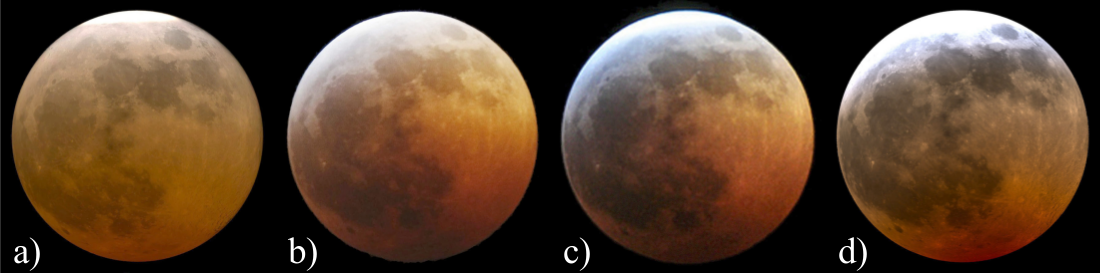
\includegraphics[width=\textwidth]{chapter01/images/Comparison_Yapo_Limberger}
    \caption{This is the image caption. The image is from Limberger et al.~\cite{Limberger2012}.}
    \label{fig:image-example}
\end{figure}


\subsection{Image Comparison}\label{subsec:image-comparison}
\begin{figure}[h]
    \begin{subfigure}[h]{0.45\textwidth}
        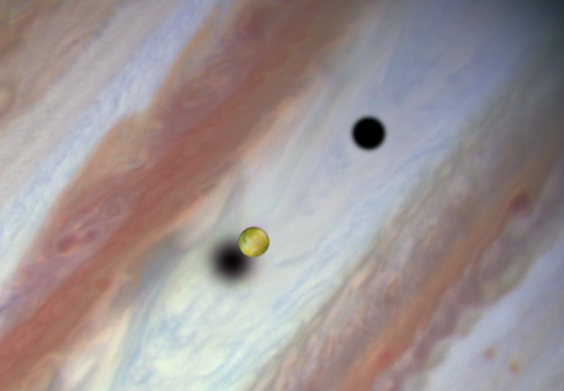
\includegraphics[width=\textwidth]{chapter01/images/HubbleJupiterEclipse2015}
    \end{subfigure}
    \hfill\vrule\hfill
    \begin{subfigure}[h]{0.45\textwidth}
        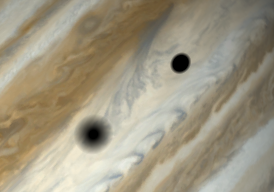
\includegraphics[width=\textwidth]{chapter01/images/CosmoGraphiaEclipseJupiter2015}
    \end{subfigure}

    \caption{Here you can see two images next to another for comparison.}
    \label{fig:image-comparison}
\end{figure}

\section{Citations and References}\label{sec:citations-and-references}
This is a citation: Limberger et al.~\cite{Limberger2012}.

This is a reference to the Appendix~\ref{ch:appendix}.

This is a reference to an image~\ref{fig:image-example}.

Here are some more citations for example purposes at the end of the paper:
\begin{itemize}
    \item Inproceedings~\cite{Yapo2009}
    \item Article~\cite{williams1978}
    \item Website~\cite{celestiaWebsite}
    \item Tech Report~\cite{usStandardAtmosphere}
    \item Master Thesis~\cite{fischer2018}
    \item Book~\cite{bohren1998}
\end{itemize}
    %\chapter{Chapter 2}\label{ch:chapter02}

\section{Formulas}\label{sec:formulas}

\begin{wraptable}{o}{0pt}
    \begin{tabular}{|r l|}
        \hline
        \multicolumn{2}{|c|}{\textbf{Symbols}} \\
        \hline
        $I$       & relative brightness \\
        $\Omega_{sun}$  & solid angle of \\
        & the sun \\
        $\Omega_{occ}$  & solid angle of \\
        & intersection \\
        \hline
    \end{tabular}
\end{wraptable}

This is a text that describes a formula.
This formula is for calculating the brightness of light for a single point that is illuminated by the sun and partially occluded by a moon.
This is done by taking the solid angle of the Sun $\Omega_{sun}$ subtracting the solid angle of the occluding moon $\Omega_{occ}$ and normalize the result.
To the right we have a table that describes all the symbols that appear on this page, so people can much more easily see what symbol has which meaning without having to reread the text everytime they want to use the formula.

\begin{equation}
    \label{eq:relative-intensity}
    I = \frac{\Omega_{sun} - \Omega_{occ}}{\Omega_{sun}}.
\end{equation}

\section{Units in Equations}\label{sec:units-in-equations}

\begin{equation}
    \frac{\SI{6371}{\kilo\meter} * \SI{149600000}{\kilo\meter}}{\SI{695510}{\kilo\meter} - \SI{6371}{\kilo\meter}} = \SI{1383000}{\kilo\meter}.\label{eq:equation-with-units}
\end{equation}

\section{Code Blocks}\label{sec:code-blocks}

This templated uses minted for formatting code.
It is required to install the python package Pygments.
You can do this with the following command: pip install Pygments

\subsection{Simple Code Block}\label{subsec:simple-code-block}

Here we can see a code block.
The second argument specifies the language for text highlighting.

\begin{minted}{c}
    // Get the intensity of the eclipse caused by the occluding body for our fragment.
    float eclipseLight = calcEclipse(occludingBody, fragPos);

    // Get the color of the fragment from the bodies texture.
    outputColor = texture(/*...*/);

    // Reduce the brightness of the fragment according to the intensity of the eclipse.
    outputColor = outputColor * eclipseLight;
\end{minted}

\subsection{Imported Code Block from File}\label{subsec:imported-code-block-from-file}

The following line imports code from a text file.
The first argument is the language for highlighting purposes.

\inputminted{c}{chapter02/code/spherical_cap_intersect.glsl}

\subsection{Inline Code}\label{subsec:inline-code}

This is inlined code: \mintinline{c}{float calcEclipse(vec4 occludingBody, vec3 fragmentPosition)}, where the first argument is the language.

\section{Tables}\label{sec:tables}

This is a table:

\begin{center}
    \begin{tabular}{ l r c r}
        \toprule
        \textbf{Body} & \textbf{Semi-major Axis} & \textbf{Observer Placement} & \textbf{Max. Abs. Error} \\
        \midrule
        Mercury & 0.39 AU & surface & 0.0008 \\
        & & 500,000km & 0.0000 \\
        \midrule
        Venus & 0.72 AU & surface & 0.0004 \\
        & & 500,000km & 0.0000 \\
        \midrule
        Earth & 1.00 AU & surface & 0.0003 \\
        & & Moon & 0.0000 \\
        \midrule
        Mars & 1.52 AU & surface & 0.0002 \\
        & & Phobos & 0.0000 \\
        & & Deimos & 0.0000 \\
        \midrule
        Jupiter & 5.20 AU & surface & 0.0000 \\
        & & Io & 0.0000 \\
        & & Callisto & 0.0000 \\
        \bottomrule
    \end{tabular}
    \captionof{table}{This is the table caption.}
    \label{tab:table-example}
\end{center}

    \appendix

    \chapter{Appendix}\label{ch:appendix}

\begin{figure}[h]
    \centering
    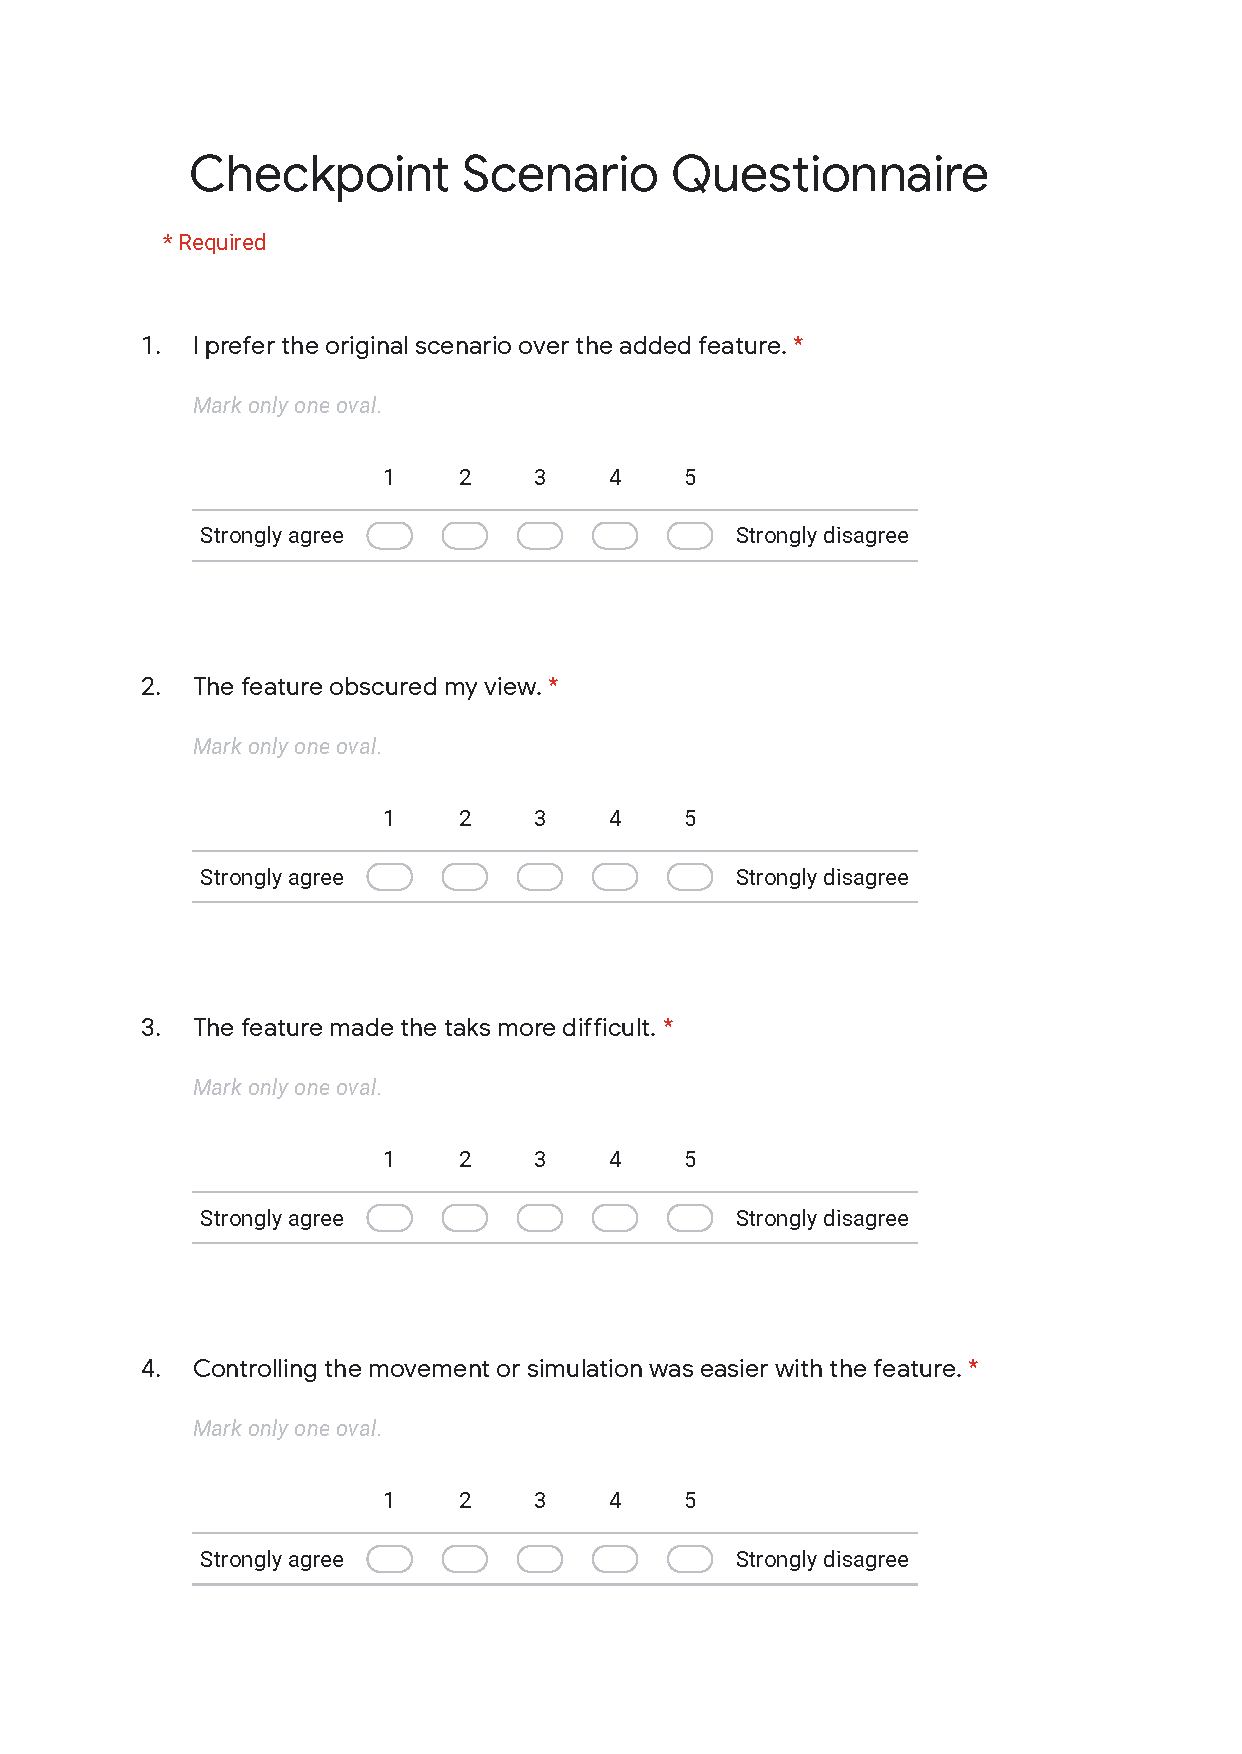
\includegraphics[width=0.8\textwidth]{content/appendix/docs/CheckpointScenarioQuestionnaire}
    \caption{Example questions for the checkpoints scenarios of the user study (page 1).}
    \label{fig:study-checkpoint-questionnaire-1}
\end{figure}

\begin{figure}[h]
    \centering
    \includegraphics[width=0.8\textwidth, page=2]{content/appendix/docs/CheckpointScenarioQuestionnaire}
    \caption{Feedback section for the checkpoints scenarios of the user study (page 2).}
    \label{fig:study-checkpoint-questionnaire-2}
\end{figure}

\begin{figure}[h]
    \centering
    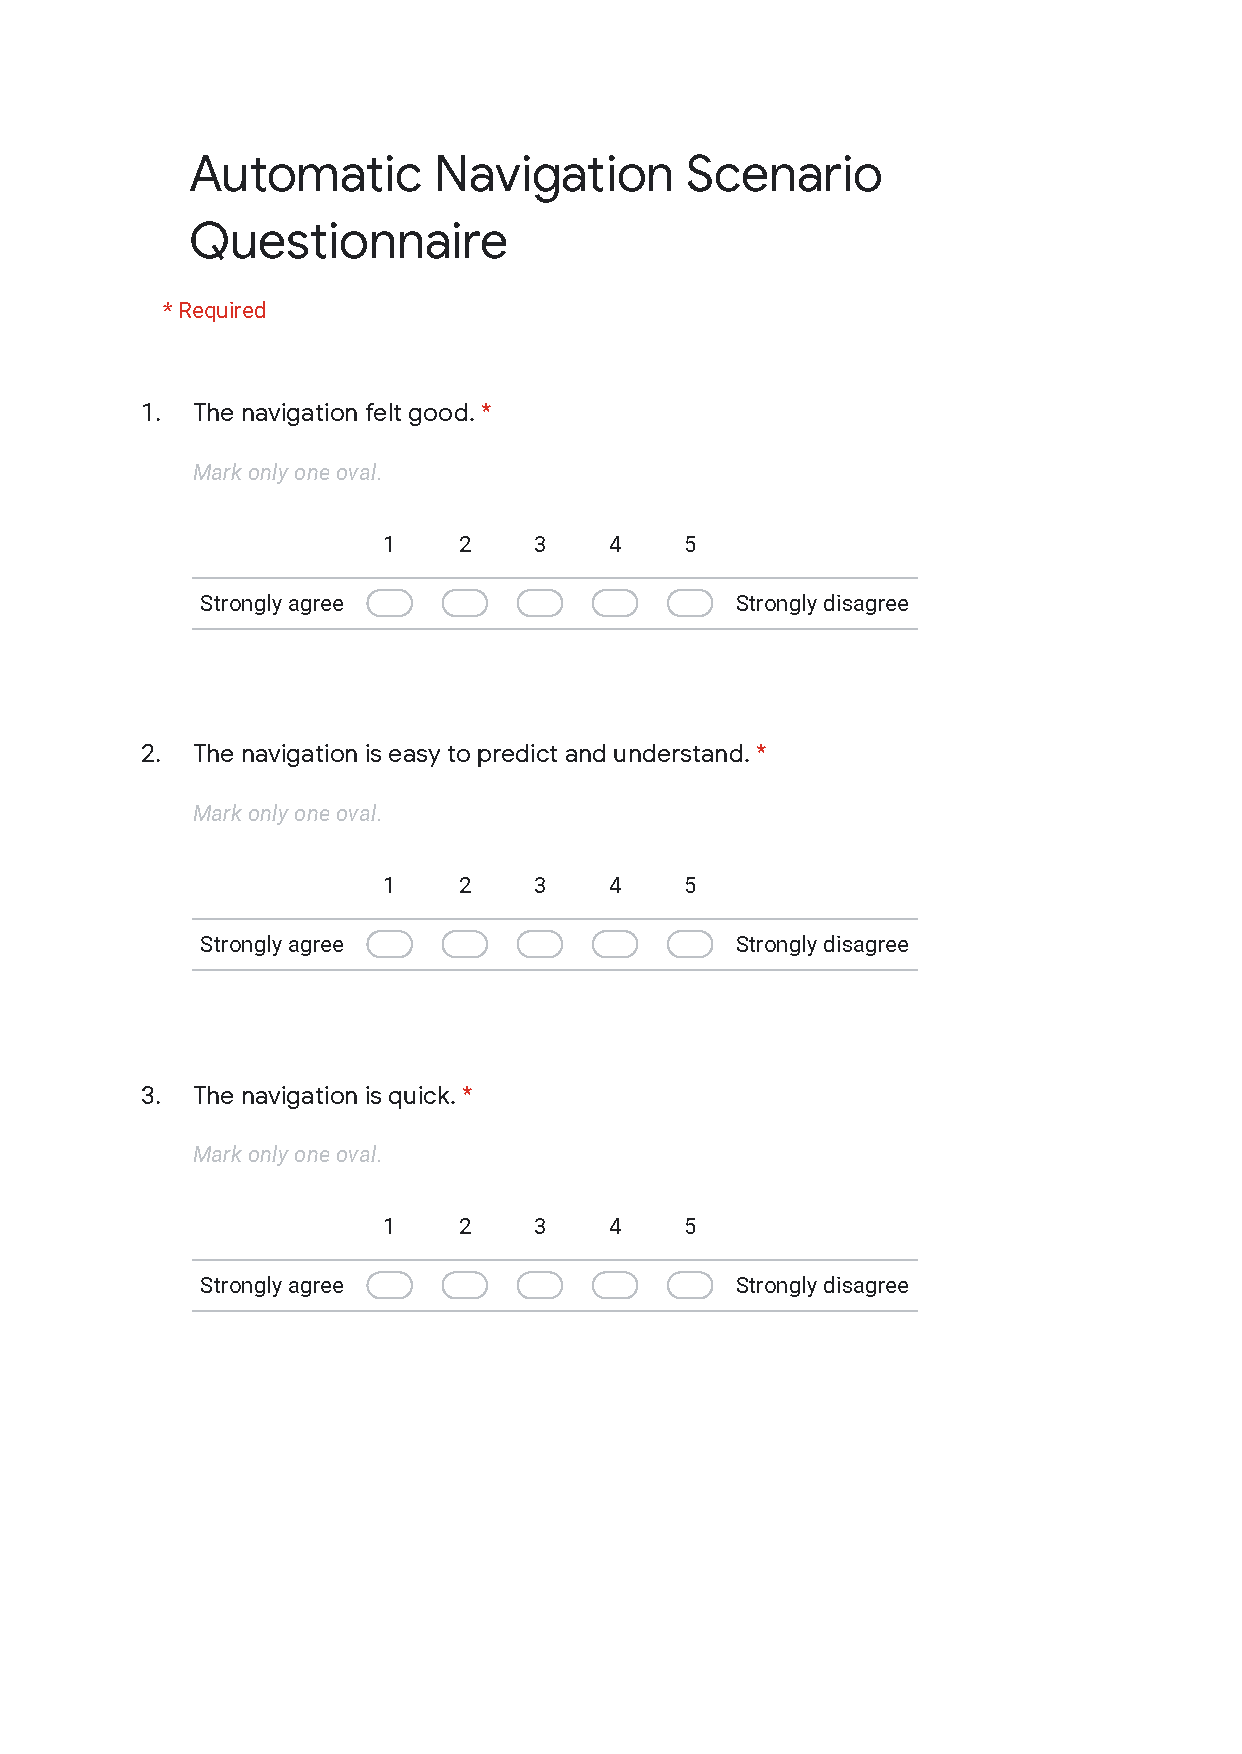
\includegraphics[width=0.8\textwidth]{content/appendix/docs/AutoNavScenarioQuestionnaire}
    \caption{Example questions for the automatic navigation scenarios of the user study (page 1).}
    \label{fig:study-autonav-questionnaire-1}
\end{figure}

\begin{figure}[h]
    \centering
    \includegraphics[width=0.8\textwidth, page=2]{content/appendix/docs/AutoNavScenarioQuestionnaire}
    \caption{Feedback section for the automatic navigation scenarios of the user study (page 2).}
    \label{fig:study-autonav-questionnaire-2}
\end{figure}


    \addcontentsline{toc}{chapter}{Bibliography}
    \renewcommand{\btxfnamespaceshort}{\,}
    \bibliographystyle{bababbrv_unsrt}
    \bibliography{main}

\end{document}
